

\newpage

%----------------------------------------------------------------------------------------

\section{An epistemological Approach}{Une Approche Epistémologique}

\label{sec:quantepistemo}


%----------------------------------------------------------------------------------------


\bpar{
A corollary of the thematic background introduced in chapter~\ref{ch:thematic} is the need of an understanding of involved disciplines themselves to be able to build integrated heterogeneous models. The potentialities of couplings and integrations are greatly determined by existing approaches and corresponding gaps.
}{
Nous avons eu un aperçu large de différents types de modèles prenant en compte les interactions entre réseaux et territoires, ainsi que les disciplines et problématiques associées. Ces aspects très différents suggèrent un cloisonnement fort des disciplines. Il reste de plus difficile de situer les modèles potentiels de co-évolution dans cette nébuleuse. Il est légitime de se demander quelles sont les relations existantes et potentielles entre les différentes approches ? Quelles domaines peuvent être passés inaperçus bien que complémentaires ?
}

% \comment[FL]{justif revue systematique algo : est-ce le pquoi de la rarete de l'intersection qui doit etre moteur ? ou de montrer les challenges a faire cette intersection et les approches les plus prometteuses ?}[les deux, connaissance de la connaissance implique connaissance]

Diverses hypothèses peuvent être avancées pour tenter d'expliquer l'absence d'investigation des modèles de co-évolution :
\begin{itemize}
	\item Suivant~\cite{commenges:tel-00923682}, les acteurs scientifiques et opérationnels qui seraient concerné par l'application pratique de tels modèles se verraient remplacés par ces mêmes modèles et donc n'ont aucune incitation à les développer (explication sociologique).
	\item Les différentes disciplines qui détiennent les diverses composantes nécessaires à de tels modèles sont cloisonnées et ont des motivations divergentes (explication épistémologique).
	\item La construction de tels modèles comporte des difficultés intrinsèques rendant leur développement décourageant.
\end{itemize}

Nous n'aurons pas les moyens d'explorer la première hypothèse (ou plutôt elle demanderait un sujet à part entière, impliquant entre autres entretiens sociologiques). La troisième est soit une tautologie soit indémontrable, à-la-Church dirait-on, et l'ensemble de notre travail permettra d'y apporter des pistes de réponse. La deuxième par contre est comme nous allons le voir plus à notre portée.



\bpar{
This implies an advanced epistemological study in each field, that we propose to tackle in a systematic and quantitative way.
}{
Une manière d'explorer cette hypothèse et de répondre aux questions précédentes consiste en une étude épistémologique que nous proposons de mener de manière quantitative et systématique. Cette approche est complémentaire de l'analyse de littérature précédente, et permet à la fois de la contextualiser et de la systématiser. Il faut par ailleurs garder en tête l'idée que l'étude des raisons de la rareté des modèles nous informera nécessairement sur les modèles eux-mêmes et les questions reliées à leur construction : la \emph{connaissance de la connaissance}~\cite{morin1986methode} accroît la connaissance.
}


\bpar{
We describe and explore first a systematic review exploration algorithm, that retrieve corpuses of references through iterative semantic extraction. We describe then briefly possible extended bibliometrics by presenting an external example of application. We finally suggest possible development directions towards unsupervised data and text-mining.
}{
Une étude préliminaire a pour but de confirmer la pertinence d'une approche d'épistémologie quantitative, en suggérant une forte isolation des disciplines. Celle-ci est menée par un algorithme de revue systématique algorithmique, qui reconstruit des corpus de références par exploration de voisinage sémantiques, c'est à dire la récupération itérative de références voisines dans leur contenu sémantique principal. Nous procédons ensuite à une analyse de réseaux, couplant réseau de citation et réseau sémantique, pour préciser les contours des disciplines impliquées. Nous suggérons finalement des possibles extensions vers de l'apprentissage non-supervisé et la fouille de texte complets pour une extraction automatique de la structure de modèles par exemple.
}



Commençons par situer le contexte des analyses en \emph{épistémologie quantitative}\footnote{Nous proposons d'utiliser ce terme pour des travaux à la croisée de la bibliométrie et de la scientométrie, des sciences cognitives, de l'épistémologie et des systèmes complexes, à l'image de l'\emph{Epistémologie Appliquée} développée jusqu'en 2011 par le laboratoire CREA.} que nous proposons de mener.




%Nous proposons de tirer parti de telles techniques pour traiter notre problème. En effet, l'observation de la bibliographie obtenue dans la section précédente soulève une hypothèse. Il semble clair que toutes les briques sont présentes pour l'existence de modèles co-évolutifs mais des questionnements et objectifs différents semblent la stopper. Des interactions restreintes entre des champs scientifiques travaillant sur les mêmes objets mais avec des objectifs et contextes divergents, et à des échelles différentes, pourrait être à l'origine de l'absence de modèles co-évolutifs.



\subsection{Quantitative epistemology}{Epistémologie quantitative}



\bpar{
The possible methods for quantitative insights into epistemology are numerous. A good illustration of the variety of approaches is given by network analysis. Using citation network features, a good predicting power for citation patterns is for example obtained by~\cite{2013arXiv1310.8220N}. Co-authorship networks can also be used for predictive models~\citep{2014arXiv1402.7268S}. A multilayer network approach was proposed in~\cite{omodei2017evaluating}, using bipartites networks of papers and scholars, in order to produce measures of interdisciplinarity using generalized centrality measures. Disciplines can be stratified into layers to reveal communities between them and therein collaboration patterns~\citep{2015arXiv150601280B}. Keyword networks are used in other fields such as economics of innovation: for example, \cite{choi2014patent} proposes a method to identify technological opportunities by detecting important keywords from the point of view of topological measures. In a similar manner, \cite{shibata2008detecting} uses topological analysis of the citation network to detect emerging research fronts.
}{
Les méthodes possibles pour des entrées quantitatives en épistémologie sont nombreuses. Une bonne illustration de la variété des approches est donnée par l'analyse de réseau. En utilisant des caractéristiques topologiques du réseau de citation, un bon pouvoir prédictif pour les motifs de citation est par exemple obtenu par~\cite{2013arXiv1310.8220N}. Les réseaux de co-auteurs peuvent également être utilisés pour des modèles prédictifs~\cite{2014arXiv1402.7268S}. Une approche par réseau multi-couches est proposée dans~\cite{omodei2017evaluating}, qui utilise des réseaux bipartites d'articles et de chercheurs, afin de produire des mesures d'interdisciplinarité en utilisant des mesures de centralité généralisées. Les disciplines peuvent être stratifiées en couches pour révéler des communautés entre celles-ci et ainsi des motifs de collaboration~\cite{2015arXiv150601280B}. Les réseaux de mots-clés sont utilisés dans d'autres champs comme en Economie de l'innovation : par exemple, \cite{choi2014patent} propose une méthode pour identifier les opportunités technologiques par la détection de mots-clés importants du point de vue des mesures topologiques. De façon similaire, \cite{shibata2008detecting} utilise une analyse topologique du réseau de citation pour détecter des fronts de recherche émergents.
}



\subsubsection{Systematic reviews}{Revues systématique}

\bpar{
Literature review is a crucial preliminary step for any scientific work and its quality and extent may have a dramatic impact on research quality. Systematic review techniques have been developed, from qualitative review to quantitative meta-analyses allowing to produce new results by combining existing studies \cite{rucker2012network}. Ignoring some references can even be considered as a scientific mistake in the context of emerging information systems~\cite{lissacksubliminal}. We aim to take advantage of such techniques to tackle our issue.
Indeed, observing the form of the bibliography obtained in previous section raises some hypothesis. It is clear that all components are present for co-evolutive models to exist but different concerns and objectives seem to stop it. As it was shown by \cite{commenges:tel-00923682} for the concept of mobility, for which a ``small world of actors'' relatively closed invented a notion ad hoc, using models without accurate knowledge of a more general scientific context, we could be in an analog case for the type of models we are interested in. Restricted interactions between scientific fields working on the same objects but with different purposes, backgrounds and at different scales, could be at the origin of the relative absence of co-evolving models. 
While most of studies in bibliometrics rely on citation networks \cite{2013arXiv1310.8220N} or co-autorship networks \cite{2014arXiv1402.7268S}, we propose to use a less explored paradigm based on text-mining introduced in~\cite{chavalarias2013phylomemetic}, that obtain a dynamic mapping of scientific disciplines based on their semantic content. For our question, it has a particular interest, as we want to understand content structure of researches on the subject. We propose to apply an algorithmic method described in the following. The algorithm proceeds by iterations to obtain a stabilized corpus from initial keywords, reconstructing scientific semantic landscape around a particular subject.
}{
Avec l'avènement des nouveaux moyens techniques et des nouvelles sources de données, la revue de littérature classique tend à se coupler à des revues automatiques. Des techniques de revue systématique ont été développées, des revues qualitatives aux meta-analyses quantitatives qui permettent de produire des nouveaux résultats par combinaison d'études existantes~\cite{rucker2012network}. Passer sous silence certaines références peut même être considéré comme une erreur scientifique dans le contexte de l'émergence des systèmes d'information qui par l'accès plus aisé à l'information rend difficilement justifiable l'omission de références clés~\cite{lissacksubliminal}\footnote{Tout en restant conscient que même avec une méthode systématique, il est impossible d'être absolument exhaustif. L'objectif est d'augmenter autant que possible la couverture, dans l'idée d'une approche inclusive de multiples points de vue, comme le propose notre positionnement épistémologique de perspectivisme donné en~\ref{sec:epistemology}.}.
}

% \comment[FL]{phrase risquee : est-tu certain de n'etre passe a cote de rien ? par exemple as tu lu Brotchie 1984 ?}[(JR) justement la est la contradiction et la justification de l'approche : maximiser couverture, tout en sachant qu'on ne peut pas tout couvrir (perspectivisme) - a developper]




\subsubsection{Interdisciplinarity}{Interdisciplinarité}


\bpar{
The development of interdisciplinary approaches is increasingly necessary for most of disciplines, both for further knowledge discovery but also societal impact of discoveries, as it was recently coined by the special issue of Nature~\citep{natureInterdisc}. \cite{banos2013pour} suggests that the development of such approaches must occur within a subtle spiral between and inside disciplines. An other way to understand this phenomenon is to understand it as the emergence of vertically integrated fields conjointly with horizontal questions as detailed in the Complex Systems roadmap (\cite{2009arXiv0907.2221B}).
}{
Le développement d'approches interdisciplinaires est de plus en plus nécessaire pour la plupart des disciplines, à la fois pour la découverte de nouvelles connaissances mais aussi pour l'impact sociétal des découvertes, comme le rappelle récemment le volume spécial de la revue Nature~\citep{natureInterdisc}. \cite{banos2013pour} suggère que leur développement doit s'insérer dans une spirale subtile entre et au sein des disciplines. Une autre façon de voir ce phénomène est de le comprendre comme l'émergence de champs verticalement intégrés\footnote{C'est à dire intégrant, généralement entre les échelles, différentes branches d'un champ : par exemple la biologie intégrative~\cite{liu2005systems} vise à des ponts entre approches génomiques, approches physiologiques, approches écologiques, en tirant parti de l'intégration des méthodes : expérimentation, modélisation, simulation.} de manière conjointe aux questions horizontales comme détaillé dans la feuille de route des Systèmes complexes (\cite{2009arXiv0907.2221B}).
}



\bpar{
There are naturally multiple views on what is exactly interdisciplinarity (many other terms such as trans-disciplinarity, cross-disciplinarity also exist) and it actually depends on involved domains : recent hybrid disciplines (see e.g. the ones underlined  by \cite{bais2010praise} such as astro-biology) are a good illustration of the case where entanglement is strong and new discoveries are vertically deep, whereas more loose fields such as ``urbanism'', which have no precise definition and where integration is by essence horizontal, are an other illustration of how transversal knowledge can be produced. Interaction between disciplines are not always smooth, as shows the misunderstandings when urban issues were recently introduced to physicists as \cite{dupuy2015sciences} recalls.
}{
Il existe naturellement de multiples points de vue sur ce qu'est exactement l'interdisciplinarité (de nombreux d'autres termes comme la trans-disciplinarité ou la cross-disciplinarité existent aussi) et cela dépend en fait des domaines impliqués : des disciplines hybrides apparues récemment (voir par exemples celles soulignées par \cite{bais2010praise} comme l'astro-biologie, ou d'autres plus proche de notre champ comme la géomatique) sont une bonne illustration du cas où les intrications sont très fortes, tandis que des champs comme ``l'urbanisme'' dont les définitions sont multiples montrent dans quelle mesure l'intégration horizontale est nécessaire et comment de la connaissance transversale peut être produite. Les interactions entre les disciplines ne sont pas toujours faciles, comme le montre les malentendus lorsque les sujets sur la ville ont été récemment introduits aux physiciens comme \cite{dupuy2015sciences} le rappelle, malentendus dont les effets peuvent être négatifs s'ils conduisent à des conflits ou à une ignorance de connaissances déjà établies par un autre domaine.
}



\bpar{
These concerns are part of an understanding of processes of knowledge production, i.e. the \emph{Knowledge of the knowledge} as \cite{morin1986methode} puts it, in which evidence-based perspectives, involving quantitative approaches, play an important role. These paradigms can be understood as a \emph{quantitative epistemology}. Quantitative measures of interdisciplinarity would therefore be part of a multidimensional approach of the study of science that is in a way ``beyond bibliometrics''~\citep{cronin2014beyond}. The focus of this paper is positioned within this stream of research. We first review existing approaches to the measure of interdisciplinarity.
}{
Ces questions font partie de la compréhension des processus de production de connaissance, i.e. la \emph{Connaissance de la connaissance} comme \cite{morin1986methode} la présente, dans laquelle les perspectives \emph{evidence-based}, qui impliquent des approches quantitatives, jouent un rôle important. Ces paradigmes peuvent être compris comme une \emph{épistémologie quantitative}. Des mesures quantitatives de l'interdisciplinarité feraient pour cette raison partie d'une approche multidimensionnelle de l'étude de la science, qui va en quelque sorte ``au delà de la bibliométrie''~\cite{cronin2014beyond}. La préoccupation de cette section se positionne dans ce champ de recherche. Nous passons d'abord en revue les approches existantes à la mesure de l'interdisciplinarité.
}



% \comment[FL]{evidence-based : traduire}[(JR)non traduisible - appuyer quelque part sur le sens de l'evidence-based]
% https://fr.wikipedia.org/wiki/M%C3%A9decine_fond%C3%A9e_sur_les_faits




\bpar{
Definitions of interdisciplinarity itself and indicators to measure it have already been tackled by a large body of literature. \cite{huutoniemi2010analyzing} recall the difference between \emph{multidisciplinary} (an aggregate of works from different disciplines) and \emph{interdisciplinary} (implying a certain level of integration) approaches. They construct a qualitative framework to classify types of interdisciplinarity, and for example distinguish empirical, theoretical and methodological interdisciplinarities. The multidimensionnal aspect of interdisciplinarity is confirmed even within a specific field such as literature~\citep{austin1996defining}. A first way to quantify interdisciplinarity of a set of publications is to look at the proportion of disciplines outside a main discipline in which they are published, as~\cite{rinia2002impact} do for the evaluation of projects in physics, complementary with judgement of experts. \cite{porter2007measuring} designate this measure as \emph{specialization}, and compares it with a measure of \emph{integration}, given by the spread of citations  done by a paper within the different Subject Categories (classification of the Web of Knowledge), which is also called the \emph{Rao-Stirling} index. \cite{lariviere2010relationship} uses it on a Web of Science corpus to show the existence of an optimal intermediate level of interdisciplinarity for the citation impact within a five year window. A similar work is done in~\citep{lariviere201410}, focusing on the evolution of measures on a long time range. The influence of missing data on this index is studied by \cite{moreno2016uncertainty}, providing an extended framework taking into account uncertainty. The use of networks has also been proposed : \cite{porter2009science} combine the integration index with a mapping technique which consists in visualisation of synthetic networks constructed by co-citations between disciplines. \cite{leydesdorff2007betweenness} shows that the betweenness centrality is a relevant indicator of interdisciplinarity, when considering appropriate citation neighborhood.
}{
Les définitions de l'interdisciplinarité elle-même et les indicateurs pour la mesurer ont déjà été traités par un vaste corpus de littérature. \cite{huutoniemi2010analyzing} rappelle la différence entre les approches \emph{multi-disciplinaires} (une agrégation de travaux de différentes disciplines) et \emph{interdisciplinaires} (qui implique un certain niveau d'intégration). Ils construisent un cadre qualitatif pour classifier différents types d'interdisciplinarité, et distinguent par exemple les interdisciplinarités empiriques, théoriques et méthodologique. L'aspect multi-dimensionnel de l'interdisciplinarité est confirmé même au sein d'un champ spécifique comme la littérature~\cite{austin1996defining}. Une première façon de quantifier l'interdisciplinarité d'un ensemble de publications est de regarder la proportion de disciplines hors d'une discipline principale dans lesquelles elles sont publiées, comme~\cite{rinia2002impact} fait pour l'évaluation de projets en physique, de manière complémentaire au jugement d'experts. \cite{porter2007measuring} désigne cette mesure comme \emph{spécialisation}, et la compare avec une mesure d'\emph{intégration} donnée par l'étendue des citations faites par un article au sein des différentes \emph{Subject Categories} (classification du \emph{Web of Knowledge}), qui est également appelé indice de \emph{Rao-Stirling}. \cite{lariviere2010relationship} l'utilise sur un corpus du \emph{Web of Science} pour montrer l'existence d'un niveau d'interdisciplinarité intermédiaire optimal pour l'impact en termes de citations sur une fenêtre de 5 ans post-publication. Un travail équivalent est fait dans~\cite{lariviere201410}, qui se concentre sur l'évolution des mesures sur une longue portée temporelle. L'influence des données manquantes sur cet index est étudié par~\cite{moreno2016uncertainty}, qui fournit un cadre étendu qui prend en compte l'incertitude. L'utilisation de réseaux a également été proposée : \cite{porter2009science} combine l'indice d'intégration avec une technique de cartographie qui consiste en la visualisation de réseaux synthétiques construits par les co-citations entre disciplines. \cite{leydesdorff2007betweenness} montre que la centralité de chemin est un indicateur pertinent d'interdisciplinarité, lorsqu'un environnement de citation pertinent est considéré.
}







%----------------------------------------------------------------------------------------



\subsection{Algorithmic Systematic Review}{Revue Systématique Algorithmique}

% Une étude bibliographique étendue suggère une rareté des modèles quantitatifs de simulation qui intègrent à la fois la croissance urbaine et la croissance des réseaux, relative à l'ensemble des modèles prenant l'un ou l'autre en compte ou qui gardent l'un statique. Cette absence pourrait être due aux intérêts divergents des acteurs des disciplines concernées qui induiraient un manque de communication.


\bpar{
A broad bibliographical study suggests a scarcity of quantitative models of simulation integrating both network and urban growth. This absence may be due to diverging interests of concerned disciplines, resulting in a lack of communication.  We propose to proceed to an algorithmic systematic review to give quantitative elements of answer to this question. A formal iterative algorithm to retrieve corpuses of references from initial keywords, based on text-mining, is developed and implemented. We study its convergence properties and do a sensitivity analysis. We then apply it on queries representative of the specific question, for which results tend to confirm the assumption of disciplines compartmentalization.
}{
Nous proposons de procéder de manière préliminaire à une revue de la littérature systématique et algorithmique. Un algorithme itératif formel pour construire des corpus de références à partir de mots-clés initiaux, basé sur l'analyse textuelle, est développé et mis en oeuvre. Nous étudions ses propriétés de convergence et procédons à une analyse de sensibilité. Nous l'appliquons ensuite à des requêtes représentatives de notre question spécifique, pour lesquelles les résultats tendent à confirmer l'hypothèse d'isolation relative des disciplines.
}


% répétition
%Nous avons revu selon divers point de vue les efforts de modélisation des interactions entre territoires et réseaux dans la section précédente~\ref{sec:modelingsa}. Cet état de l'art nous suggère fortement des domaines relativement cloisonnés et s'intéressant à des problématiques différentes. Une question naturelle est alors celle de l'existence de modèles endogénéisant la co-évolution, i.e. prenant en compte simultanément la croissance urbaine et celle du réseau. Nous essayons d'y répondre par une revue systématique algorithmique.


Tandis que la majorité des études en bibliométrie se reposent sur les réseaux de citation~\cite{2013arXiv1310.8220N} ou les réseaux de co-auteurs~\cite{2014arXiv1402.7268S}, nous proposons d'utiliser un paradigme moins exploré, basé sur l'analyse textuelle, introduit par~\cite{chavalarias2013phylomemetic}, qui produit une cartographie dynamique des disciplines scientifiques en se basant sur leur contenu sémantique. Nous prenons le parti d'une appréhension de la diversité des domaines, introduite en~\ref{sec:modelingsa}, par cette information supplémentaire du paysage scientifique. Les méthodes que nous introduisons sont particulièrement adaptées pour notre étude puisque nous voulons comprendre la structure du contenu des recherches sur le sujet.

%Nous appliquons une approche algorithmique décrite par la suite.



%\paragraph{Description of the Algorithm}{Description de l'Algorithme}

%%%%%%%%%%%%%%%%%%%%%%%%%%%%
%\paragraph{Results}{Résultats}

% description donnée en annexe

L'algorithme procède par itérations pour obtenir un corpus stabilisé à partir de mots-clés initiaux, reconstruisant l'horizon sémantique scientifique autour d'un sujet donné. La description formelle de l'algorithme est détaillée en Annexe~\ref{app:sec:quantepistemo}, avec les détails de son implémentation et des analyses de sensibilité. Sa logique est donnée par le schéma en Fig.~\ref{fig:quantepistemo:algo} : étant donné un ensemble de mots-clés de départ que l'on rassemble en une unique requête, on récolte des travaux qui en traitent, dont on extrait de nouveaux mots-clés pour itérer en boucle jusqu'à convergence éventuelle.

%%%%%%%%%%%%%%%%%%%%%%%%%%%%
\begin{figure}
\centering
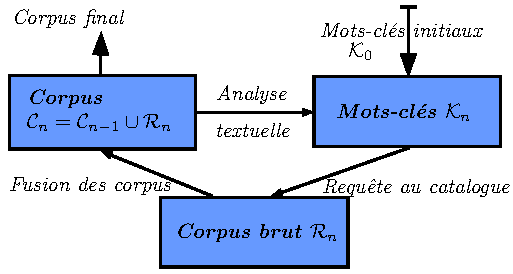
\includegraphics[width=0.8\linewidth]{Figures/QuantEpistemo/schema_algo}
\caption[Systematic review algorithm workflow][Algorithme de revue systématique]{Global workflow of the algorithm, including implementation details: catalog request is done through Mendeley API; final state of corpuses are RIS files.\label{fig:quantepistemo:algo}}{\textbf{Architecture globale de l'algorithme.} A partir d'un ensemble de mots-clés initiaux, on construit un corpus par requête au catalogue, duquel on extrait des nouveaux mots-clés par analyse textuelle. On itère alors en boucle jusqu'à obtenir un corpus fixe ou dépasser un nombre maximal fixé d'itérations.\label{fig:quantepistemo:algo}}
\end{figure}
%%%%%%%%%%%%%%%%%%%%%%%%%%%%



%\bpar{
%Once the algorithm is partially validated, we apply it to our question.
%}{
%Les détails précis concernant l'implémentation de l'algorithme ainsi qu'une analyse de sensibilité pour vérifier la convergence sur un échantillon de requêtes initiales sont donnés en Appendice~\ref{app:sec:quantepistemo}. Cette analyse permet de donner confiance en sa robustesse, puisqu'on a convergence rapide (moins d'une cinquantaine d'itérations) pour l'ensemble des requêtes testées et des différentes valeurs pour $N_k$.\comment[AB]{et alors ? est-ce peu ?} Nous proposons alors de l'appliquer à notre question.
%}

%\comment[FL]{mots-cles en entree : tu pars de l'anglais, c'est un choix fort, a preciser ; pourquoi pas des mots simples ? pourquoi ces mots-l ? (pas coevolution) : c'est crucial}[explicite en notes de bas de page]

\bpar{
We start from five different initial requests that were manually extracted from the various domains identified in the bibliography (that are ``city system network'', ``land use transport interaction'', ``network urban modeling'', ``population density transport'', ``transportation network urban growth''). We take the weakest assumption on parameter $N_k=100$, as it should less constrain reached domains. After having constructed corpuses, we study their lexical distances as an indicator to answer our initial question. Large distances would go in the direction of the assumption made above, i.e. that discipline self-centering may be at the origin of the lack of interest for co-evolutive models. We show in Table~\ref{tab:quantepistemo:lexical} values of relative lexical proximity, that appear to be significantly low, confirming this assumption.

}{
Nous partons de cinq différentes requêtes initiales qui ont été manuellement extraites des divers domaines identifiés dans la bibliographie\footnote{Qui sont ``cityANDsystemANDnetwork'', ``land-useANDtransportANDinteraction'', ``networkANDurbanANDmodeling'', ``populationANDdensityANDtransport'', ``transportationANDnetworkANDurbanANDgrowth''. Ce choix inclut les approches par systèmes de villes, les approches LUTI, les approches de croissance de réseau. Il ne peut bien sûr être exhaustif. Cette étude étant préliminaire on admet de travailler potentiellement sur des échantillons. Par exemple, l'utilisation de ``co-evolution'' n'est pas concluante car trop peu d'articles utilisent cette formulation. De même, la question de la langue conditionne les résultats : une requête en Français conduit à des niches linguistiques finalement assez pauvres en diversité, et nous faisons ainsi uniquement des requêtes en anglais. L'approche par hyper-réseau développée plus loin sera elle multilingue.}, afin de comparer les corpus obtenus pour chaque requête. Après avoir construit les corpus, nous étudions leur cohérence lexicale comme un indicateur de réponse à notre question initiale. De grande distances devraient confirmer l'hypothèse formulée ci-dessus, i.e. que des disciplines auto-centrées pourraient être à l'origine d'un manque d'intérêt pour des modèles co-évolutifs. La table~\ref{tab:quantepistemo:lexical} montre les valeurs de la proximité lexicale relative, que nous définissons par un indice de similarité d'ensemble pondéré donné par
\[
d(I,J) = \frac{\sum_{k_i \in I, k_j \in J} \mathbbm{1}_{k_i = k_j} \cdot (s(k_i) + s(k_j))}{\sum_{k_i \in I} s(k_i) + \sum_{k_j \in J} s(k_j)}
\]
%\comment[JR]{pas du tout explicite : def du score ? meilleure ref à l'annexe}
pour les corpus $I,J$, et avec $s$ fonction strictement positive donnant une mesure d'importance des mots au sein des corpus fournie par la méthode d'extraction des mots-clés (voir~\ref{app:sec:quantepistemo}). Ses valeurs sont significativement faibles en comparaison à la valeur de référence 1 pour des corpus égaux (la mesure s'interprète comme une proportion de mots en co-occurrence), ce qui tend à confirmer notre hypothèse\footnote{Pour situer ces résultats de manière relative, il faudrait un modèle nul (c'est à dire générateur de corpus avec distributions sémantiques similaires mais sans structure de corrélation entre mots) avec des corpus aléatoires par exemple, ce qui pourrait faire l'objet de développements futurs.}.
}

% \sum 1_{words equals} * score_ki + score_kj / (sum score_i + sum score_j) -> sorte de Jaccard pondéré.



%%%%%%%%%%%%%%%%%%%%%%%%%%%%
\begin{table}
\caption[Stationary lexical proximities][Proximités lexicales stationnaires]{Symmetric matrix of lexical proximities between final corpuses, defined as the sum of overall final keywords co-occurrences between corpuses, normalized by number of final keywords (100). We obtain very low values, confirming that corpuses are significantly far. Size of final corpuses is given as $W$.\label{tab:quantepistemo:lexical}}{Matrice symétrique des proximités lexicales entre les corpus finaux, définies comme la somme des co-occurrences pondérées de mots-clés finaux entre corpus, normalisé par le poids total des mots-clés finaux. La taille des corpus finaux est donnée par $W$. Les valeurs obtenues pour les proximités sont considérablement faibles par rapport à la valeur maximale 1, ce qui confirme que les corpus sont éloignés de manière significative.\label{tab:quantepistemo:lexical}}
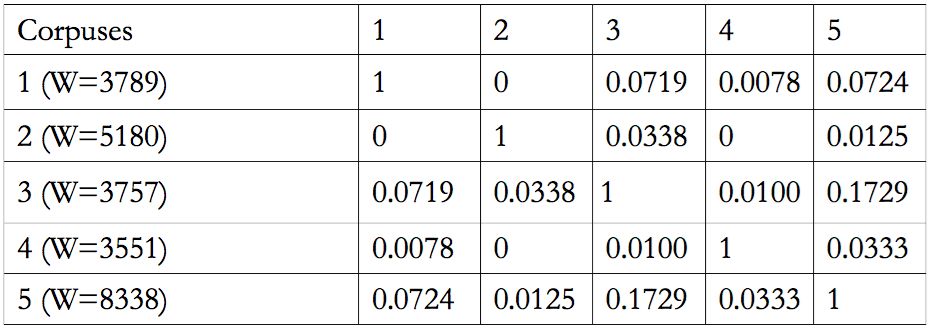
\includegraphics[width=0.8\linewidth]{Figures/QuantEpistemo/corpusesDistances}
% \comment[FL]{ce tableau est difficilement comprehensible ; traduire ; trop de chiffres significatifs.}
% \comment[AB]{C’est vrai que sans valeurs de références c’est difficile à interpréter. Quelle serait la valeur max pour un corpus de taille X et un nombre de mots clés Y ?}
% \comment[JR]{nom des corpus ?}
\end{table}
%%%%%%%%%%%%%%%%%%%%%%%%%%%%




%\bpar{
%Possible developments can include the construction of citation networks through an automatic access to Google Scholar that provides backward citations. The confrontation of inter-cluster coefficients on the citation network for the different corpuses with lexical consistence are an essential aspect of a further validation of our results.
%}{
%Les développements possibles incluent la construction de réseaux de citation via un accès automatique à Google Scholar\comment[FL]{pourquoi cette plateforme et pas une autre ?} \comment[AB]{c’est ton unique source ?
%Si je fais une recherche à la main dans google scholar avec les termes « urban growth networks » j’obtiens des références, par exemple 
%Streets tree networks and urban growth: optimal geometry for quickest access between a finite-size volume and one point
%A Bejan, GA Ledezma - Physica A: Statistical Mechanics and its …, 1998} qui fournit les citations entrantes. La confrontation des coefficients inter-clusters pour le réseau de citations entre les différents corpus avec la cohérence lexicale est un aspect clé d'une validation approfondie des résultats.
%}





\bpar{
The disturbing absence of models simulating the co-evolution of transportation networks and urban land-use, confirmed through a state-of-the-art covering many domain, may be due to the absence of communication between scientific disciplines studying different aspects of that problems. We have proposed an algorithmic method to give elements of answers through text-mining-based corpus extraction. First numerical results seem to confirm the assumption. However, such a quantitative analysis should not be considered alone, but rather come as a back-up for qualitative studies that will be the object of further work, such as the one lead in~\cite{commenges:tel-00923682}, in which questionnaires with historical actors of modeling provide highly relevant information.
}{
La constatation d'un faible nombre de modèles qui simulent la co-évolution des réseaux de transport et de l'usage du sol urbain pourrait être due à l'absence de communication entre les disciplines scientifiques étudiant différents aspects du problème. D'autres explications possibles qui en sont proches peuvent par exemple être le manque de cas d'application concrets de tels modèles vu les échelles temporelles mises en jeu et donc l'absence de financement propre - ce qui n'est pas si loin de l'absence d'une discipline y consacrant certains de ses objets. Cette question des portées et des échelles des modèles fera l'objet de la meta-analyse à la section suivante~\ref{sec:modelography}. Ainsi, nous avons proposé ici une méthode algorithmique pour donner des éléments de réponse par l'extraction de corpus basée sur l'analyse textuelle, dont les résultats numériques semblent aller dans le sens d'une compartimentalisation des disciplines (au sens particulier utilisé ici d'une distance sémantique entre corpus niches). Cette analyse était relativement limitée dans la portée de ses résultats, notamment par le faible nombre de requêtes et un certain nombre d'incertitudes intrinsèques, mais est \emph{suffisante} pour produire un diagnostic, à savoir (i) une structure disciplinaire fortement marquée peut être extraite de l'analyse de corpus, et (ii) l'utilisation d'outils sémantique permet une extraction d'information endogène. Fort de ce diagnostique préliminaire, nous proposons d'approfondir l'analyse par une variation et extension de la méthode employée.
}


%\comment[JR]{Expliciter ce que conduit la suite : le premier traitement est un diagnostique, puis plus solide ensuite.}



%--------------------------------------------------------------


%%%%%%%%%%%%%%%%%%%%%%%%
%\subsection[Indirect Bibliometrics][Bibliométrie indirecte]{Indirect bibliometrics through Complex Network analysis}{Bibliométrie Indirecte par Analyse de Réseaux Complexes}
\subsection{Indirect Bibliometrics}{Bibliométrie indirecte}

\label{subsec:indirectbibliometrics}


\bpar{
As described before, semantic analysis of final corpus does not contain all the information on disciplinary compartmentation nor on patterns of propagation of scientific knowledge as the ones contained in citation networks for example. Furthermore, data collection in the previous algorithm is subject to convergence towards self-consistent themes because of the proper structure of the method. It may give more insight about scientific social patterns of ontological choices in modeling to study communities in broader networks, that would more correspond to disciplines (or sub-disciplines depending on granularity level). We propose to reconstruct disciplines around our thematic, to obtain a more precise view of interdisciplinarity and the scientific landscape on our subject.
}{
Comme décrit précédemment, l'analyse sémantique des corpus finaux ne contient pas la totalité de l'information sur les liens entre disciplines ni sur les motifs de propagation de la connaissance scientifique comme ceux contenus dans les réseaux de citations par exemple. De plus, la collection des données dans l'algorithme précédent est sujette à convergence vers des thèmes relativement auto-cohérents de par la structure propre de la méthode. On pourrait obtenir plus d'information sur les motifs sociaux de choix ontologiques pour la modélisation en étudiant les communautés dans des réseaux plus larges, ce qui correspondrait plus à des disciplines (ou des sous-disciplines selon le niveau de granularité). Nous proposons de reconstruire les disciplines autour de notre thématique, pour obtenir une vue plus précise du paysage scientifique sur notre sujet et des liens entre disciplines. Une contribution fondamentale de cette section consiste en la construction de jeux de données hybrides à partir de sources hétérogènes, et les développement des outils associés qui peuvent être réutilisés et améliorés pour des applications similaires. Cette démarche peut être vue comme une bibliométrie indirecte\footnote{La bibliométrie, ou scientométrie lorsqu'elle est appliquée en particulier à la science comme dans notre cas, consiste en la mesure et la qualification des motifs de production de connaissance par l'intermédiaire de leur supports directement observables (productions scientifiques, fonctionnement des institutions, relations sociales entre chercheurs, etc.)~\cite{cronin2014beyond}. Cet ouvrage rappelle que ce domaine est en pleine mutation et dresse une carte des nouvelles approches.}, puisqu'on cherche à reconstruire une information endogène et à extraire des relations entre différentes dimensions.
}

% \comment[FL]{est ce que si les disciplines sont (re) construites par l'algo, la notion d'interdisciplinarite a le meme sens ?}[pertinent -> peut etre ne pas appeler cela interdisc / discussion avec Geoffrey Caruso et Marion Maisonnabe][cf discussion papier cybergeo annexe]


\subsubsection{Context}{Contexte}




\bpar{
The approach developed here couples citation network exploration and analysis with text-mining, aiming at mapping the scientific landscape in the neighborhood of a particular corpus. The context is particularly interesting for the methodology developed. First of all, the subject studied is very broad and by essence interdisciplinary. Secondly, bibliographical data is difficult to obtain, raising the concern of how the perception of a scientific landscape may be shaped by actors of the dissemination and thus far from objective, making technical solutions as the ones consequently developed here crucial tools for an open and neutral science.
}{
L'approche développée ici couple exploration et analyse de réseau de citation avec analyse textuelle, dans le but de cartographier le paysage scientifique dans le voisinage d'un corpus donné. Le contexte est particulièrement intéressant pour la méthodologie développée. Premièrement, le sujet étudié est très large et par essence interdisciplinaire. Deuxièmement, les données bibliographiques sont difficiles à obtenir, soulevant la question de comment la perception d'un horizon scientifique peut être déterminée par les acteurs de la dissémination et donc loin d'être objective, rendant les solutions techniques comme celle développée ici en conséquence des outils cruciaux pour une science ouverte et neutre.
}

\bpar{
Our approach combine semantic communities analysis (as done in~\cite{2016arXiv160208451P} for papers in physics but with keyword extraction ; \cite{2015arXiv151003797G} analyses semantic networks of political debates) with citation network to extract e.g. interdisciplinarity measures. Our contribution differs from the previous works quantifying interdisciplinarity as it does not assume predefined domains nor classification of the considered papers, but reconstructs from the bottom-up the fields with the endogenous semantic information. \cite{nichols2014topic} already introduced a close approach, using Latent Dirichlet Allocation topic modeling to characterize interdisciplinarity of awards in particular sciences. \cite{lariviere201410} quantifies interdisciplinarity over a long time range by looking at the field of references of publications.
}{
Notre approche combine une analyse des communautés sémantiques (comme fait dans~\cite{2016arXiv160208451P} pour les articles en physique mais sans extraction des mots-clés, ou par \cite{2015arXiv151003797G} pour un analyse des réseaux sémantiques de débats politiques) avec celle du réseau de citations pour extraire par exemple des mesures d'interdisciplinarité. Cette contribution se démarque des travaux précédents quantifiant l'interdisciplinarité puisqu'elle ne suppose pas de domaines a priori ou une classification des références considérées, mais reconstruit par le bas les champs via l'information sémantique endogène. \cite{nichols2014topic} introduit une approche similaire, utilisant le modèle d'extraction de thématiques \emph{Latent Dirichlet Allocation}\footnote{Le modèle LDA, introduit par~\cite{blei2003latent}, suppose les documents comme produits par des thèmes sous-jacents, avec une distribution de Dirichlet pour leur composition ainsi que pour la distribution des mots par thèmes. Son estimation donne la composition des thèmes en terme de mots-clés.} pour caractériser l'interdisciplinarité de récompenses dans des sciences précises.
}



%%%%%%%%%%%%%%%%%%%%%%%
\subsubsection{Database Construction}{Données}


\bpar{
Our approach imposes some requirements on the dataset used, namely: (i) cover a certain neighborhood of the studied journal in the citation network in order to have a consistent view on the scientific landscape; (ii) have at least a textual description for each node. For these to be met, we need to gather and compile data from heterogeneous sources, using therefore a specific application, which general architecture is synthesized in Fig.~\ref{fig:datacollection}. For the sake of simplicity, we will denote by \emph{reference} any standard scientific production that can be cited by another (journal paper, book, book chapter, conference paper, communication, etc.) and contains basic records (title, abstract, authors, publication year). We will work in the following on networks of references. Note that one significant contribution of this paper is the construction of such an hybrid dataset from heterogeneous sources, and the development of associated tools that can be reused and further developed for similar purposes.
}{
Notre approche implique des spécifications pour le jeu de données utilisé, à savoir : (i) couvrir un voisinage conséquent du corpus étudié dans le réseau de citation afin d'avoir une vue la moins biaisée possible du paysage scientifique ; (ii) avoir au moins une description textuelle pour chaque noeud. Pour cela, nous rassemblons et compilons les données de sources hétérogènes en utilisant une architecture et implémentation spécifiques, décrites en Appendice~\ref{app:sec:cybergeo}. Pour simplifier, nous dénommons \emph{référence} toute production scientifique standard\footnote{Ce qui est bien sûr sujet à débat, voir nos discussions en ouverture sur l'évolution des modes de communication scientifique.} qui peut être citée par une autre (articles de journaux, livre, chapitre de livre, article d'actes, communication, etc.) et contient des informations de base (titre, résumé, auteurs, année de publication). Nous travaillons par la suite sur le réseau des références.
}

\paragraph{Initial Corpus}{Corpus Initial}

Notre corpus initial est construit à partir de l'état de l'art établi en~\ref{sec:modelingsa}. Sa composition complète est donnée en Appendice~\ref{app:sec:quantepistemo}. Celui-ci est pris de taille raisonnable (conduisant à un réseau final traitable sans méthode spécifique concernant la taille des données), mais les méthodes utilisées ici ont été développées sur des données massives, pour les brevets par exemple~\cite{bergeaud2017classifying}.


\paragraph{Citation Data}{Données de citation}

\bpar{
Citation data is collected from \texttt{Google Scholar}\comment[FL]{police}, that is the only source for incoming citations~\cite{noruzi2005google} in our case as the journal is poorly in other databases\footnote{or was just added as in the case of \textit{Web of Science}, indexing \textit{Cybergeo} since May 2016}. We are aware of the possible biaises using this single source (see e.g.~\cite{bohannon2014scientific})\footnote{or \texttt{http:\/\/iscpif.fr\/blog\/2016\/02\/the-strange-arithmetic-of-google-scholars}}, but these critics are more directed towards search results than citation counts. %The automatic collection requires the use of an open source data crawling software to pipe requests, namely \texttt{TorPool}~\cite{torpool} that provides a Java API allowing an easy integration into our application. Using it, a crawler can retrieve html pages and get backward citation data, i.e. all citing articles for a given initial article.
 We retrieve that way two sub-corpuses: references \emph{citing} Cybergeo and references \emph{citing the ones cited} by cybergeo. At this stage, the full corpus contains around $4\cdot10^5$ references.
}{
Le réseau de citations est reconstruit à partir de \texttt{Google Scholar} qui est souvent l'unique source des citations entrantes~\cite{noruzi2005google} puisqu'en science humaines les ouvrages ne sont pas systématiquement référencés par les bases fournissant des services (payants) comme le réseau de citation.\footnote{Par exemple, le journal Cybergeo n'est indexé dans le \emph{Web of Science} que depuis mai 2016, suite à des négociations ardues et non sans contrepartie.} Nous sommes conscient des biais possibles de l'utilisation de cette source unique (voir par exemple~\cite{bohannon2014scientific})\footnote{ou \texttt{http://iscpif.fr/blog/2016/02/the-strange-arithmetic-of-google-scholars}}, mais ces critiques sont dirigées vers les résultats de recherche plutôt que les comptes de citations. Nous récoltons ainsi les références \emph{citantes} à profondeur deux, c'est à dire les références citant le corpus initial et celles citant celles-ci. Le réseau obtenu contient $V=9462$ références correspondant à $E=12004$ liens de citation. Concernant les langues, l'anglais représente 87\% du corpus, le français 6\%, l'espagnol 3\%, l'allemand 1\%, complété par des langues comme le mandarin pouvant être indéfinies (la détection de celui-ci étant peu fiable). %Le corpus n'est pas très international (contrairement par exemple au thème de la croissance urbaine, étudié pour le développement thématique sur les liens entre économie et géographie développé en~\ref{app:sec:ecogeo}). % ! finalement pas fait ! : temps pour ça ?
%\comment[JR]{presenter en bullet ou en tableau}[pour les langues ? bof..]
}

\paragraph{Text Data}{Données textuelles}

\bpar{
A textual description for all references is necessary for a complete semantic analysis. We use for this an other source of data, that is the online catalog of \textit{Mendeley} reference manager software~\cite{mendeley}. It provides a free API allowing to get various records under a structured format. Although not complete, the catalog provides a reasonable coverage (over 55\%), yielding a final corpus with full abstracts of size $2.1\cdot 10^5$, which structure is recalled in Fig.~\ref{fig:citationnetwork}
}{
Pour mener l'analyse sémantique, une description suffisamment conséquente est nécessaire. Nous collectons pour cela les résumés pour le réseau précédent. Ceux-ci sont disponibles pour environ un tiers des références, donnant $V=3510$ noeuds avec description textuelle.
}



%%%%%%%%%%%%%%%%%%
\subsubsection{Results}{Résultats}

%\comment[FL]{il faut d'abord presenter le corpus plus en detail et des resultats basique, tu commences par des choffres impossibles a mettre en contexte}



\paragraph{Citation Network Properties}{Réseau de citations}


Des statistiques basiques pour le réseau de citation donnent déjà des informations intéressantes. Le réseau a un degré moyen de $\bar{d}=2.53$ et une densité de $\gamma=0.0013$\footnote{Pour référence, \cite{batagelj2003efficient} présente les caractéristiques de 11 réseaux scientifiques de domaines divers et de taille allant de 40 à 8851 noeuds, et reporte des densité variant de $3.3\cdot 10^{-4}$ à $0.038$, avec une médiane à $0.003$, proche de celle de notre réseau.}. Le degré entrant moyen (qui peut être interprété comme un facteur d'impact stationnaire) est de 1.26, ce qui est relativement élevé pour des sciences humaines. Il est important de noter sa connexité faible, ce qui signifie que les domaines initiaux ne sont pas en isolation totale : les références initiales sont partagées à un degré minimal par les différents domaines. Nous travaillons sur la suite sur le sous-réseau des noeuds comprenant au moins deux liens, pour extraire le coeur de la structure du réseau et se débarrasser de l'effet ``grappe''. De plus, le réseau est nécessairement complet entre ces noeuds puisqu'on est remonté au deuxième niveau.


Nous procédons pour le réseau de citation à une détection de communautés par l'algorithme de Louvain, sur le réseau non-dirigé correspondant. L'algorithme fournit 13 communautés, de modularité dirigée 0.66\footnote{La modularité est une mesure du ``niveau de clustering'' d'une partition d'un réseau en classes. L'algorithme de Louvain construit les communautés par optimisation gourmande de la modularité.}, extrêmement significative en comparaison à une estimation par bootstrap de la même mesure sur le graphe aléatoirement rebranché qui donne une modularité de $0.0005 \pm 0.0051$ sur $N=100$ répétitions. Les communautés font sens de manière thématique, puisqu'on retrouve pour les plus grosses les domaines présentés dans le tableau suivant :

\medskip
\begin{center}
\begin{tabular}{|l|l|}
\hline
	Domaine & Taille (\% de noeuds)\\\hline
	LUTI & 18\% \\\hline
	Géographie Urbaine et des Transports & 16\% \\\hline
	Planification des infrastructures & 12\% \\\hline
	Planification intégrée - TOD & 6\% \\\hline
	Réseaux Spatiaux & 17\% \\\hline
	Etudes d'accessibilité & 18\% \\\hline
\end{tabular}
\end{center}
\medskip

Les appellations sont à regard d'expert a posteriori, selon les grands domaines dégagés dans la revue de littérature en~\ref{sec:modelingsa}\footnote{On note que cette dénomination est bien exogène et nécessairement subjective. Comme développé plus loin pour le réseau sémantique, il n'existe pas de technique simple pour une désignation endogène. Il faut garder cet aspect en tête pour la mise en perspective des interprétations et conclusions.}.


La Fig.~\ref{fig:quantepistemo:citnw} montre le réseau de citation et permet de visualiser les relations entre ces domaines. Il est intéressant d'observer que les travaux des économistes et des physiciens dans le domaine tombent dans la même catégorie d'étude des \emph{Spatial Networks}. En effet, la littérature citée par les physiciens comporte souvent plus d'ouvrage en économie qu'en géographie, tandis que les économistes utilisent des techniques d'analyse de réseau. Ensuite, le planning, l'accessibilité, les LUTI et le TOD sont très proches mais se distinguent dans leur spécificités : le fait qu'ils apparaissent dans des communautés séparées témoigne d'un certain niveau de cloisonnement. Ceux-ci font le pont entre les approches Réseaux spatiaux et les approches géographiques, qui comportent une partie importante de sciences politiques par exemple. Les liens entre physique et géographie restent très faibles. Ce panorama dépend bien sûr du corpus initial, mais nous permet de mieux comprendre le contexte de celui-ci dans son environnement disciplinaire.


%%%%%%%%%%%%%%%%%
\begin{figure}[!ht]
%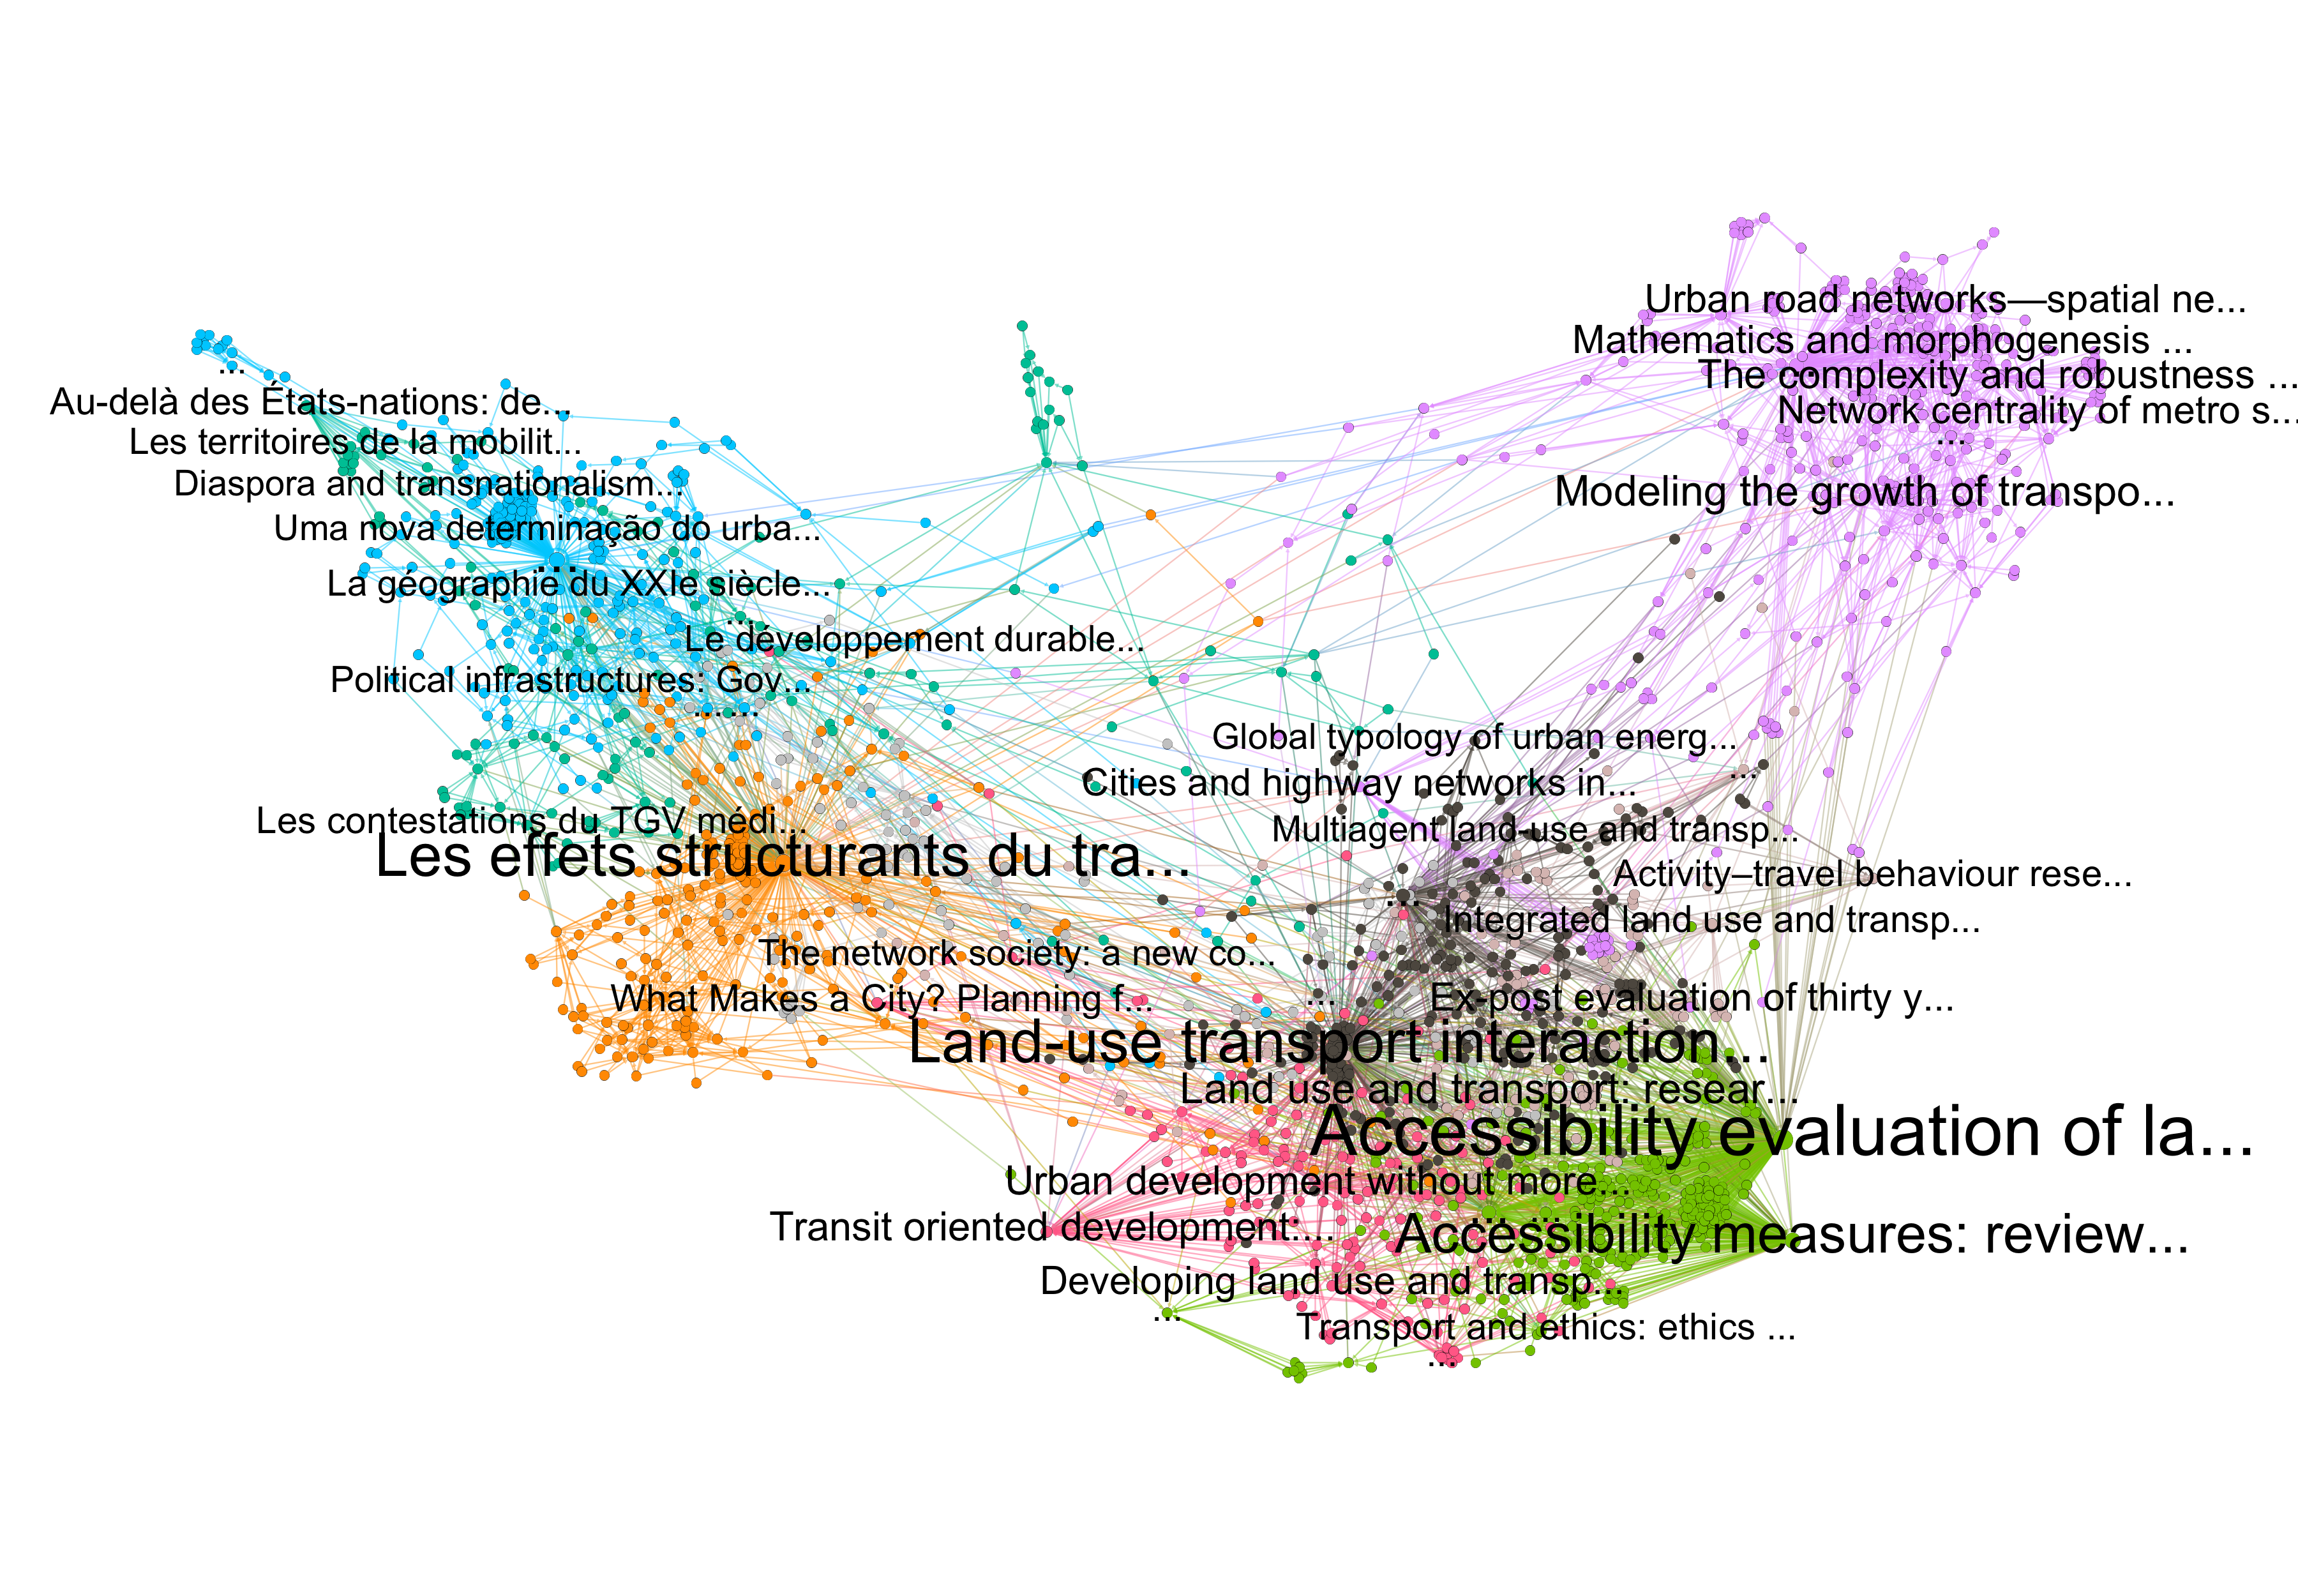
\includegraphics[width=\linewidth]{Figures/QuantEpistemo/rawcore_labs36.png}
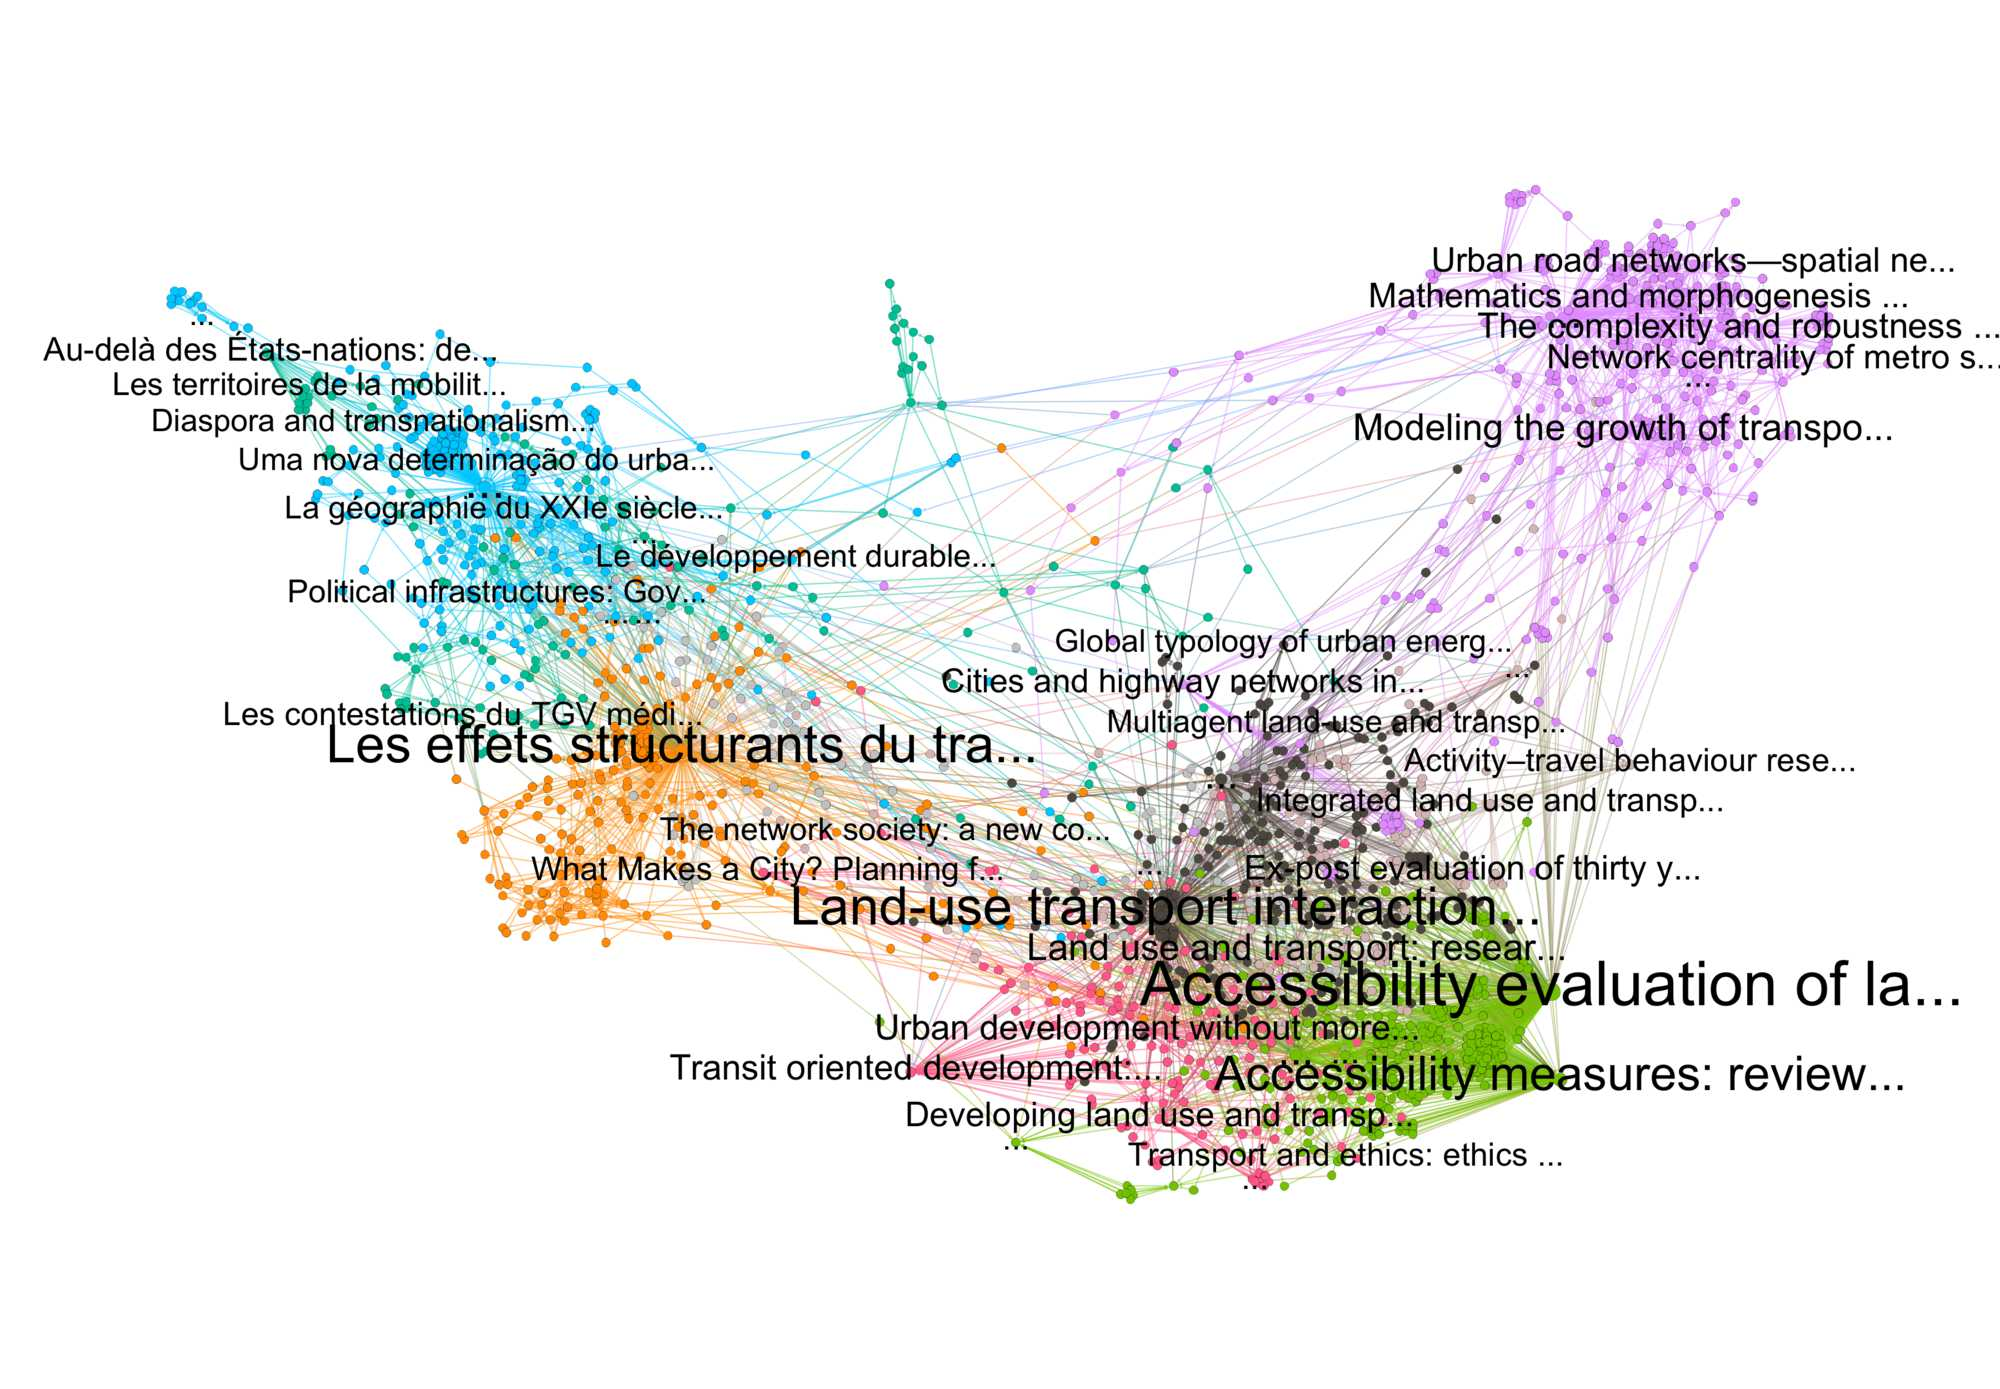
\includegraphics[width=\linewidth]{Figures/Final/2-2-2-fig-quantepistemo-citnw.jpg}
\caption[Citation Network][Réseau de citations]{\textbf{Citation Network}\label{fig:quantepistemo:citnw}}{\textbf{Réseau de citations.} Nous visualisons les références ayant au moins deux liens, par un algorithme de force-atlas. Les couleurs donnent les communautés décrites dans le texte. En orange, bleu, turquoise: géographie urbaine, géographie des transports, sciences politiques ; en rose, noir, vert: planning, accessibilité, LUTI ; en violet : réseaux spatiaux (physique et économie).\label{fig:quantepistemo:citnw}}
\end{figure}
%%%%%%%%%%%%%%%%%





%%%%%%%%%%%%%%%%%%
\paragraph{Semantic Communities}{Communautés Sémantiques}


L'extraction des mots-clés est faite suivant une heuristique inspirée de~\cite{chavalarias2013phylomemetic}. La description complète de la méthode et de son implémentation est donnée en Appendice~\ref{app:sec:cybergeo}. Elle se base sur les relations au second ordre entre les entités sémantiques, qui sont des \emph{n-grams}, c'est à dire des mots-clés multiples pouvant avoir une longueur jusqu'à 3. Celles-ci sont estimées via la matrice de co-occurrence, dont les propriétés statistiques fournissent une mesure de déviation à des co-occurrences uniformes, qui est utilisée pour juger la pertinence des mots-clés. Sélectionnant un nombre fixe de mots-clés pertinents $K_W = 10000$, nous pouvons ensuite construire un réseau pondéré par les co-occurrences.


\bpar{
The topology of raw networks does not allow the extraction of clear communities, in particular because of the presence of hubs that correspond to frequent terms common to many fields (e.g. \texttt{model}, \texttt{space}). We assume these highest degree terms do not carry specific information on particular classes and can be thus filtered given a maximal degree threshold $k_{max}$. Similarly, edge with small weight are considered as noise and filtered according to a minimal edge weight threshold $\theta_w$. Keywords are preliminary filtered by a document frequency window $\left[ f_{min},f_{max} \right]$ which is slightly different from network filtering and complementary. A sensitivity analysis of resulting network topology to these parameters is presented in Fig.~\ref{fig:sensitivity}. We choose parameter values that maximize modularity under the constraint of a community number and size distribution of same magnitude as technological classes. This multi-objective optimization does not have a unique solution as objectives are somehow contradictory, and a compromise point must be chosen.
}{
La topologie du réseau brut ne permet pas l'extraction claire de communautés, en particulier à cause de hubs qui correspondent à des termes fréquents commun à de nombreux champs (e.g. \texttt{model}, \texttt{space}). Ces mots sont utilisés de manière comparable dans l'ensemble des champs étudiés, et ne portent pas d'information pour les séparer\footnote{Mais en porteraient si l'on comparait un corpus de géographie quantitative et un corpus de musicologie par exemple.}. Nous faisons l'hypothèse que ces termes à fort degré ne portent pas d'information particulière sur des classes données et peuvent ainsi être filtrés étant donné un seuil de degré maximal $k_{max}$ (on s'intéresse alors à ce qui fait la spécificité de chaque domaine). De la même manière, les liens avec un poids faibles sont considérés comme du bruit et filtrés selon un seuil de poids minimal $\theta_w$. La méthode générique permet de plus une filtration préliminaire des mot-clés, complémentaire à la filtration topologique, par fréquence d'apparition dans les documents $\left[ f_{min},f_{max} \right]$, à laquelle les résultats ne sont pas sensibles dans notre cas. L'analyse de sensibilité des caractéristiques du réseau filtré, notamment de sa taille, modularité et structure des communautés, est donnée en~\ref{app:sec:quantepistemo}. Nous choisissons des valeurs de paramètres permettant une optimisation multi-objectifs entre modularité et taille du réseau, $\theta_w = 10,k_{max} = 500$, par le choix d'un point compromis sur un front de Pareto, qui donne un réseau sémantique de taille $(V=7063,E=48952)$. Celui-ci est visualisé en Appendice~\ref{app:sec:quantepistemo}.
}


\bpar{
We then retrieve communities in the semantic network (using standard Louvain algorithm, with the optimized filtering parameters). communities correspond to well-defined scientific fields (and/or domains, approaches). An expert validation allow us to give names to these, a more complicated naming procedure would eventually be possible (as in~\cite{yang2000improving} for the case of patents 
 where a chi-square test on distribution of documents in classes), but we prefer to stick here to a certain level of supervision. Table~\ref{tab:domains} summarizes the communities 
}{
Nous récupérons ensuite les communautés dans le réseau par un clustering de Louvain standard sur le réseau filtré optimal. On obtient 20 communautés pour une modularité de 0.58. Celles-ci sont examinées à la main pour être nommées, les techniques de désignation automatique~\cite{yang2000improving} ne sont pas assez élaborées pour faire la distinction implicite entre champs thématiques et méthodologiques par exemple (en fait entre les domaines de connaissance, voir~\ref{sec:knowledgeframework}) qui est une dimension supplémentaire que nous ne traitons pas ici, mais nécessaire pour avoir des désignations parlantes. Les communautés sont décrites en Table~\ref{tab:quantepistemo:semanticdomains}. On voit tout de suite la complémentarité avec l'approche par citations, puisque se dégagent ici à la fois des sujet d'étude (High Speed Rail, Maritime Networks), des domaines et méthodes (Networks, Remote Sensing, Mobility Data Mining), des domaines thématiques (Policy), des méthodes pures (Agent-based Modeling, Measuring). Ainsi, une référence peut mobiliser plusieurs de ces communautés. On a de plus une granularité plus fine de l'information. L'effet du langage est puissant puisque la géographie française se distingue en une catégorie séparée (des analyses poussées pourraient être envisagées pour mieux comprendre le phénomène et en tirer parti: sous-communautés, reconstruction d'un réseau spécifique, études par traduction ; mais celles-ci sont hors de propos dans cette étude exploratoire). On constante l'importance des réseaux, des problématiques de sciences politiques et socio-économiques. Nous mobiliserons la première catégorie dans la plupart des modèles développés, mais en gardant en tête l'importance des problématiques liées à la gouvernance, nous réaliserons un travail spécifique en~\ref{sec:lutetia}.
}




%%%%%%%%%%%%%%%%%%
\begin{table}
\caption[Semantic communities][Communautés sémantiques]{Disciplines/domains/fields reconstructed from community detection in the semantic network}{\textbf{Description des communautés sémantiques.} On donne leur taille, leur proportion en quantité de mots-clés (sous la forme de \emph{multi-stems})  cumulés sur l'ensemble du corpus, et des mots-clés représentatifs sélectionnés par degré maximal.\label{tab:quantepistemo:semanticdomains}}
\begin{tabular}{llll}
\hline\noalign{\smallskip}
Name & Size & Weight & Keywords  \\
\noalign{\smallskip}\hline\noalign{\smallskip}
Networks & 820 & 13.57\% & \texttt{social network, spatial network, resili} \\
Policy & 700 & 11.8\% & \texttt{actor, decision-mak, societi} \\
Socio-economic & 793 & 11.6\% & \texttt{neighborhood, incom, live} \\
High Speed Rail & 476 & 7.14\% & \texttt{high-spe, corridor, hsr} \\
French Geography & 210 & 6.08\% & \texttt{système, développement, territoire} \\
Education & 374 & 5.43\% & \texttt{school, student, collabor} \\
Climate Change & 411 & 5.42\% & \texttt{mitig, carbon, consumpt} \\
Remote Sensing & 405 & 4.65\% & \texttt{classif, detect, cover} \\
Sustainable Transport & 370 & 4.38\% & \texttt{sustain urban, travel demand, activity-bas} \\
Traffic & 368 & 4.23\% & \texttt{traffic congest, cbd, capit} \\
Maritime Networks & 402 & 4.2\% & \texttt{govern model, seaport, port author} \\
Environment & 289 & 3.79\% & \texttt{ecosystem servic, regul, settlement} \\
Accessibility & 260 & 3.23\% & \texttt{access measur, transport access, urban growth} \\
Agent-based Modeling & 192 & 3.18\% & \texttt{agent-bas, spread, heterogen} \\
Transportation planning & 192 & 3.18\% & \texttt{transport project, option, cba} \\
Mobility Data Mining & 168 & 2.49\% & \texttt{human mobil, movement, mobil phone} \\
Health Geography & 196 & 2.49\% & \texttt{healthcar, inequ, exclus} \\
Freight and Logistics & 239 & 2.06\% & \texttt{freight transport, citi logist, modal} \\
Spanish Geography & 106 & 1.26\% & \texttt{movilidad urbana, criteria, para} \\
Measuring & 166 & 1.0\% & \texttt{score, sampl, metric} \\
\noalign{\smallskip}\hline
\end{tabular}
\end{table}
%%%%%%%%%%%%%%%%%%



%%%%%%%%%%%%%%%%%%
\paragraph{Measures of Interdisciplinarity}{Mesures d'interdisciplinarité}


\bpar{
Distribution of keywords within communities provides an article-level interdisciplinarity.
Combination of citation and semantic layers in the hyper-network provide second order interdisciplinarity measures, that we don't use here because of the modest size of the citation network. More precisely, a reference can be viewed as a probability vector on semantic classes.
}{
La distribution des mots clés dans les communautés permettent de définir une mesure d'interdisciplinarité au niveau de l'article. La combinaison des couches de citation et sémantique dans l'hyperréseau fournit des mesures d'interdisciplinarité au second ordre (motifs sémantiques des cités ou des citants), que nous n'utiliserons pas ici à cause de la taille modeste du réseau de citation (voir \ref{app:sec:cybergeo} et \ref{app:sec:patents}). Plus précisément, une référence $i$ peut être vue comme un vecteur de probabilités sur les classes sémantiques $j$, qu'on notera sous forme matricielle $\mathbf{P}=(p_{ij})$. Celles-ci sont estimées simplement par les proportions de mots-clés classifiés dans chaque classe pour la référence. Une mesure classique d'interdisciplinarité~\cite{bergeaud2017classifying} est alors $I_i = 1 - \sum_j p_{ij}^2$. Soit $\mathbf{A}$ la matrice d'adjacence du réseau de citation, et soit $\mathbf{I}_k$ les matrices de selection des lignes correspondants à la classe $k$ de la classification de citation: $Id\cdot \mathbbm{1}_{c(i)=k}$, telle que $I_k \cdot A \cdot I_{k'}$ donne exactement les citations de $k$ vers $k'$. La proximité de citation entre les communautés de citation est alors définie par $c_{kk'} = \sum \mathbf{I}_k \cdot \mathbf{A} \cdot \mathbf{I}_{k'} /  \sum \mathbf{I}_k \cdot \mathbf{A}$. On définit la proximité sémantique en définissant une matrice de distance entre références par $\mathbf{D} = d_{ii'}=\sqrt{\frac{1}{2}\sum (p_{ij}-p{i'j})^2}$ puis la proximité sémantique par $s_{kk'} = \mathbf{I}_k \cdot \mathbf{D} \cdot \mathbf{I}_{k'} / \sum \mathbf{I}_k \sum \mathbf{I}_{k'}$.
}



\bpar{}{
Nous montrons en Fig.~\ref{fig:quantepistemo:interdisc} les valeurs de ces différentes mesures, ainsi que la composition sémantique des communautés de citation, pour les classes sémantiques majoritaires. La distribution de $I_i$ montre que les articles gravitant dans le domaine du LUTI sont les plus interdisciplinaires dans les termes utilisés, ce qui pourrait être lié à leur caractère appliqué. Les autres disciplines sont dans des motifs similaires, à part la géographie et la planification des infrastructures qui présentent des distributions quasi-uniformes, témoignant de l'existence de références très spécialisées dans ces classes. Ce n'est pas nécessairement étonnant vu les sous-champs pointus exhibés (sciences politiques par exemples, et de même les études prospectives type coût-bénéfices sont très étriquées). Ce premier croisement des couches nous confirme les spécificités de chaque champ. Concernant les compositions sémantiques, la plupart agissent comme validation externe vu les classes majoritaires. Le champ le moins concerné par les problème socio-économiques est la planification des infrastructure, ce qui donnera du grain à moudre aux détracteurs de la technocratie. Les questions de changement climatique et durabilité sont relativement bien répartie. Enfin, les ouvrages géographiques concernent en majorité des problèmes de gouvernance.
}


\bpar{}{
Les matrices de proximité confirment la conclusion obtenue précédemment en termes de citation, les partages étant très faibles, les plus hautes valeurs étant jusqu'à un quart de la planification vers la géographie et des LUTI vers le TOD (mais pas l'inverse, les relations peuvent être à sens unique). Hors, les proximités sémantiques montrent par exemple que LUTI, TOD, Accessibility et Networks sont proches dans leur termes, ce qui est logique pour les trois premiers, et confirme pour le dernier que les physiciens se basent majoritairement sur les méthodes des ces champs liés au planing pour légitimer leur travaux. La géographie est totalement isolée, sa plus proche voisine étant la planification des infrastructures. Cette étude est très utile pour notre propos, puisqu'elle montre des domaines cloisonnés partageant des termes et donc a priori des problématiques et sujet commun. Les domaines ne se parlent pas toute en parlant des languages pas si lointains, d'où la pertinence accrue de vouloir accorder leur partitions dans nos travaux : nos modèles devront mobiliser des éléments, ontologies et échelles de ces différents champs.
}



%%%%%%%%%%%%%%%%%%
\begin{figure}
%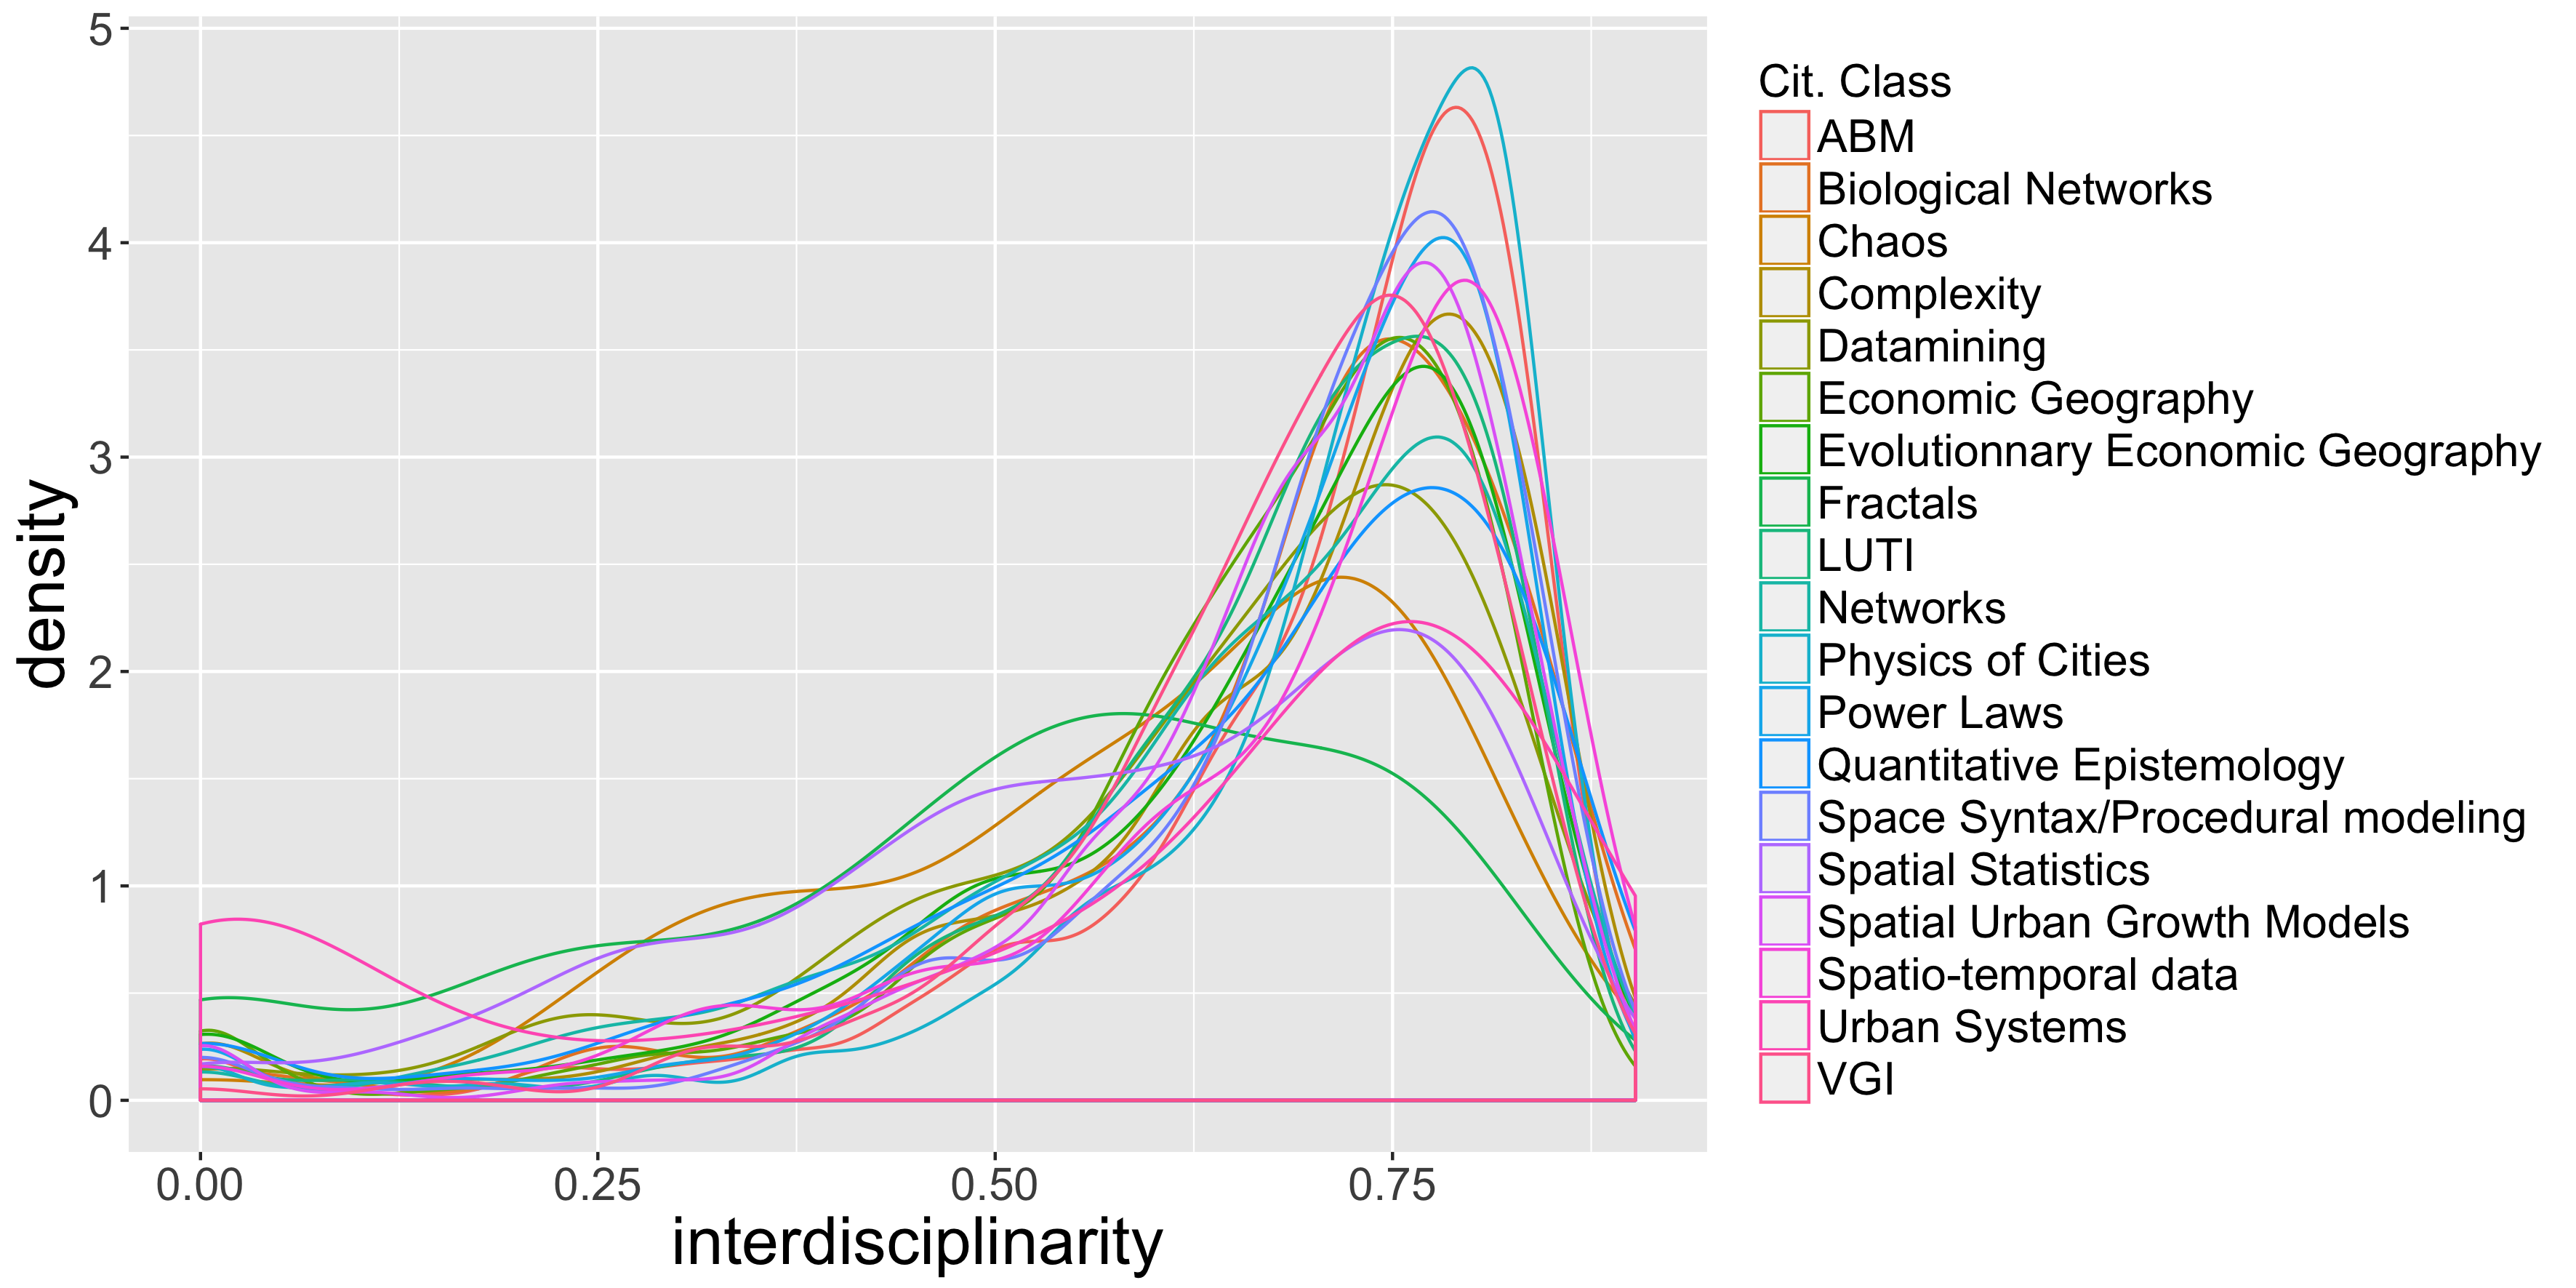
\includegraphics[width=0.49\linewidth]{Figures/QuantEpistemo/interdisciplinarities}
%\includegraphics[width=0.49\linewidth]{Figures/QuantEpistemo/compo_proportion}\\
%\includegraphics[width=0.49\linewidth]{Figures/QuantEpistemo/citation_proximities}
%\includegraphics[width=0.49\linewidth]{Figures/QuantEpistemo/semantic_proximities}
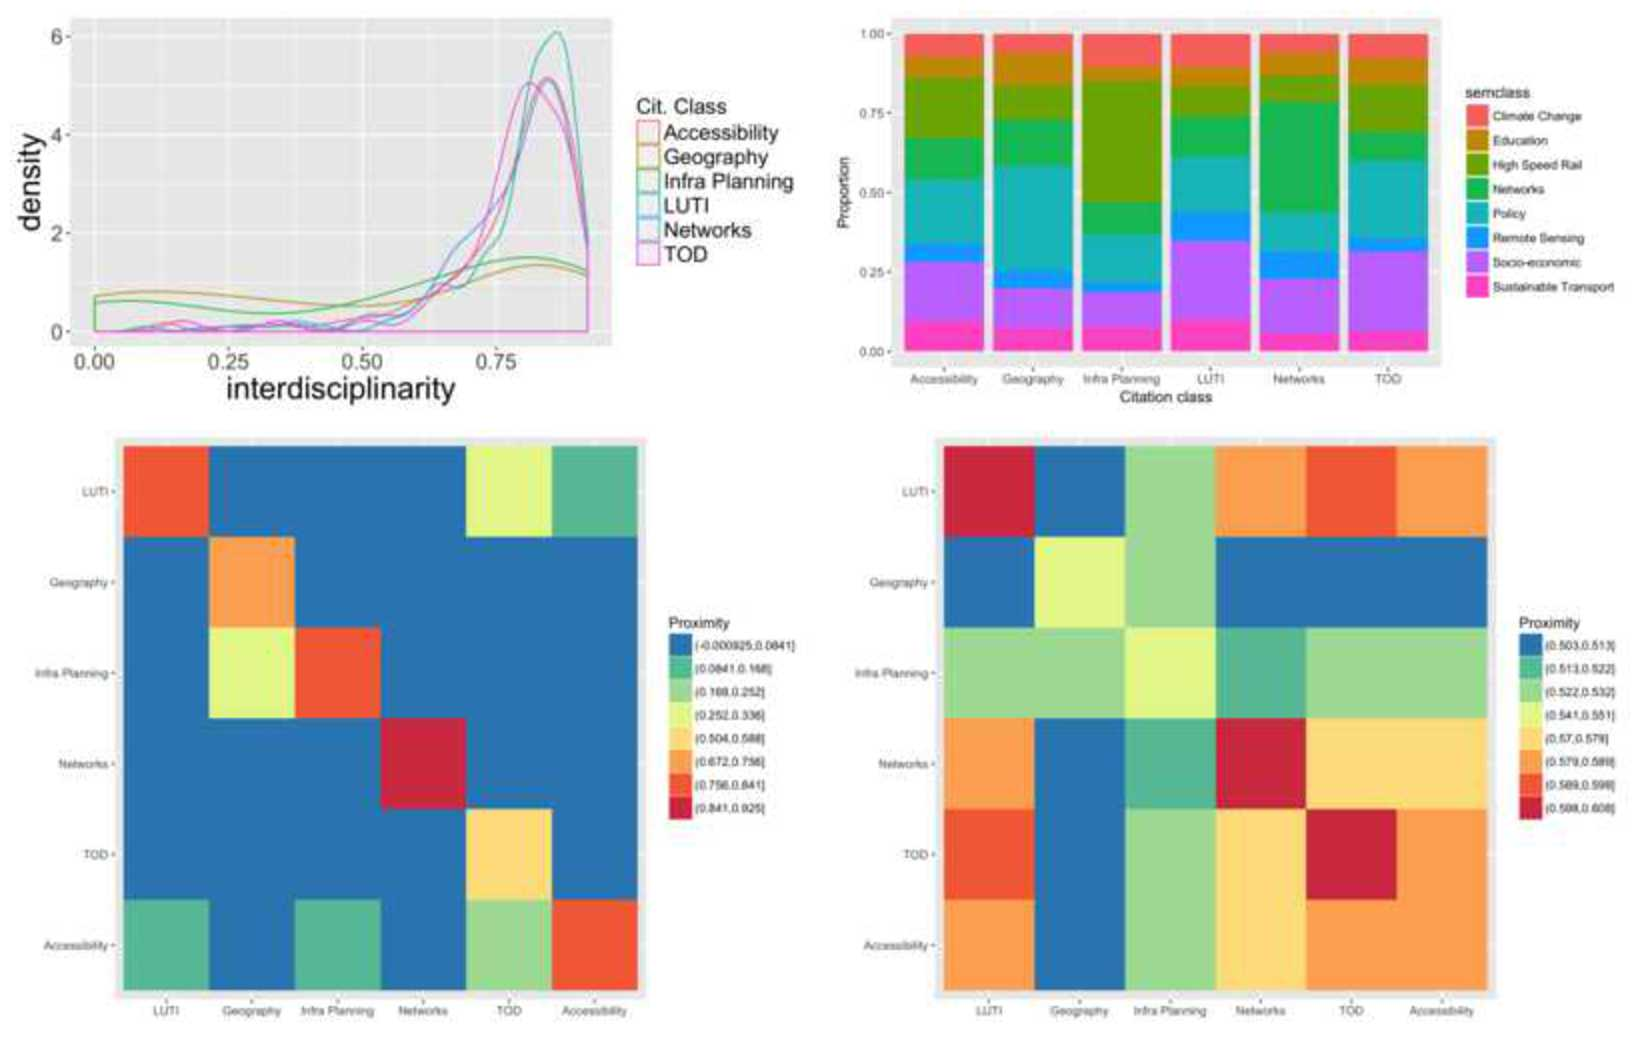
\includegraphics[width=\linewidth]{Figures/Final/2-2-2-fig-quantepistemo-interdisc.jpg}
\caption[][Motifs d'interdisciplinarité]{\label{fig:quantepistemo:interdisc}}{\textbf{Motifs d'interdisciplinarité.} \textit{(Haut Gauche)} Distribution statistique des $I_i$ par classes de citations, en d'autre termes répartition des niveaux d'interdisciplinarité au sein des classes de citation ; \textit{(Haut Droite)} Composition sémantiques des classes de citation : pour chaque classe de citation (en abscisse), la proportion de chaque classe sémantique (en couleur) est donnée ; \textit{(Bas Gauche)} Matrice de proximité de citation $c_{kk'}$ entre classes de citations ; \textit{(Bas Droite)} Matrice de proximité sémantique $s_{kk'}$ entre classes de citations.\label{fig:quantepistemo:interdisc}}
%\comment[FL]{de seconde importance je crois. sous cette forme : a synthetiser}[c'est central !]
%\comment[FL]{bien expliquer mais categories (?) dans figure 8 : curieux}[pourquoi ?]
\end{figure}
%%%%%%%%%%%%%%%%%%



% bootstrap
%min(corrs);max(corrs);mean(abs(corrs))
% -0.170952  0.5496791  0.08384802
% apply(bcorrs,2,mean)
%       minrho        maxrho    meanabsrho     minrhosup     maxrhosup meanabsrhosup 
%  -0.08792137    0.11690677    0.03137750   -0.17686637    0.68579406    0.11079253 
% apply(bcorrs,2,sd)
%       minrho        maxrho    meanabsrho     minrhosup     maxrhosup meanabsrhosup 
%  0.012683338   0.021324056   0.002250636   0.038402781   0.134996447   0.051553244 

% modularities
% sem : 0.1053156
% cit : 0.8140818
% bootstrap N=100
% sem : 0.073097051446193 +- 0.00307154703966512
% cit : 0.204223565075042 +- 0.0141450119581389


\bpar{
}{
Nous concluons cette analyse par une approche plus robuste pour quantifier les proximités entre couches de l'hyperréseau. Il est aisé de construire une matrice de corrélation entre deux classifications, par les corrélations de leur colonnes. Nous définissons les probabilités $\mathbf{P}_C$ toutes égales à 1 pour la classification de citation. La matrice de correlation de celle-ci avec $\mathbf{P}$ s'étend de -0.17 à 0.54 et a une moyenne de valeur absolue de 0.08, ce qui est significatif par rapport à des classifications aléatoire puisque un bootstrap à $b=100$ répétitions avec les matrices mélangées donne un minimum à $-0.08 \pm 0.012$, un maximum à $0.11 \pm 0.02$ et une moyenne absolue à $0.03 \pm 0.002$. Cela montre que les classifications sont complémentaires et que cette complémentarité est significative statistiquement par rapport à des classifications aléatoires. L'adéquation de la classification sémantique par rapport au réseau de citation peut également être quantifiée par la modularité multi-classes~\cite{nicosia2009extending} (voir~\ref{app:sec:patentsmining} pour une définition mathématique), qui traduit la probabilité qu'un lien soit dû à la classification étudiée, en prenant en compte l'appartenance simultanée à de multiples classes. Ainsi, la modularité multi-classes des probabilités sémantiques pour le réseau de citation est de 0.10, ce qui d'une part est significativement signe d'adéquation, un bootstrap toujours à $b=100$ donnant une valeur de $0.073 \pm 0.003$, qui reste limitée vu la valeur maximale fixée par les probabilités de citations dans leur propre réseau qui donnent une valeur de 0.81, ce qui confirme d'autre part la complémentarité des classifications.
}


%\comment[FL]{tu compares les disciplines entre elles mais pas la facon dont elles attaquent les questions au coeur de ta these. c'est dommage.}[(JR)c'est l'objet de la section suivante]


\bpar{}{
Nous avons ainsi dressé dans cette section un aperçu des disciplines en relation avec notre sujet, ainsi que leur relations. Il s'agira dans la section suivante de comprendre avec plus de détail leur ``contenu'', c'est-à-dire les moyens mobilisés pour résoudre les problèmes rencontrés.
}






%--------------------------------------------------------------


\subsubsection{Discussion}{Discussion}

Donnons brièvement des directions d'extension de l'analyse que nous venons de mener ainsi que des implications pour le positionnement épistémologique de notre travail.



\subsubsection{Towards modeling purpose and context automatic extraction}{Vers une modélisation des thèmes et une extraction automatique du contexte}


\bpar{
A possible direction to strengthen our quantitative epistemological analysis would be to work on full textes related to the modeling of interaction between networks and territories, with the aim to automatically extract thematics within articles. The idea would be to perform some kind of automatized modelography, with possible features to be extracted that would be ontologies, model architecture or structures, scales, or even typical parameter values. It is not clear to what degree structure of models can be extracted from their description in papers and it surely depends on the discipline considered. For example in a framed field such as transportation planning, using a pre-defined ontology (in the sense of dictionary) and a fuzzy grammar could be efficient to extract information as the discipline is relatively formatted. In theoretical and quantitative geography, beyond the barrier of language, information organisation is surely less subject to unsupervised data-mining because of the more literary nature of the discipline : synonyms and figures of speech are generally the norm in good level human sciences writing, fuzzing a possible generic structure of knowledge description. 
}{
Une direction possible pour renforcer cette analyse en épistémologie quantitative serait de travailler sur les textes complets des références contenant des efforts de modélisation des interactions entre réseaux et territoires, avec le but d'extraire automatiquement les thématiques des articles. Des méthodes plus adaptées pour les long texte que celle utilisée ici incluent par exemple l'Allocation Latente de Dirichlet~\cite{blei2003latent}. L'idée serait de procéder à une sorte de modélographie automatique, étendant la méthodologie de modélographie développée par~\cite{schmitt2013modelographie}, pour extraire des caractéristiques telle les ontologies, l'architecture ou la structure des modèles, les échelles ou même des valeurs typiques des paramètres. Il n'est pas clair dans quelle mesure la structure des modèles peut être extraite de leur description dans un article, et cela dépend sûrement de la discipline considérée. Par exemple dans un champ relativement cadré comme la planification des transports, l'utilisation d'une ontologie pré-définie (dans le sens d'un dictionnaire) et d'une grammaire floue pourrait être efficace vu les conventions assez strictes dans la discipline. En géographie théorique et quantitative, au-delà de la barrière de la diversité des formalisations possibles pour une même ontologie, l'organisation de l'information est sûrement plus délicate à appréhender par de l'apprentissage non-supervisé à cause de la nature plus littéraire de la discipline : les synonymes et les figures de style sont généralement la norme pour l'écriture d'un bon niveau en sciences humaines, rendant plus floue une possible structure générique de la description des connaissances.
}


%Depending on extended results of the two previous sections and on thematic requirements (huge need of knowledge on precise models structure, that may appear when trying to construct more specialized operational models), this project may be conducted with more or less investment.



% dev quali / interviews ?

%Cependant, une telle analyse quantitative ne doit pas être considérée seule, mais doit bien être comprise comme précision de la revue de littérature menée précédemment. D'autre part, elle pourrait aussi être complémentaire à des études qualitatives et des entretiens avec acteurs historiques qui peuvent être l'objet de développements futurs, comme par exemple dans l'étude menée par~\cite{commenges:tel-00923682}.


\subsubsection{Reflexivity}{Réflexivité}


\bpar{
The methodology developed here is particularly interesting since it is reflexive, i.e. it can be used on our work itself. Therefore, an other application will be the reflexivity of our thesis : we attend to proceed to similar analysis on our proper bibliography (and possibly its evolution, available via \texttt{git} history), to understand our patterns of knowledge, possible gaps or unveil unexpected developments. The detailed development is done in Appendix~\ref{app:reflexivity}.
}{
La méthodologie que nous avons développé ici est efficace pour offrir des instruments de réflexivité, c'est à dire qu'elle peut être utilisée pour étudier notre approche elle-même. Une de ses applications, hors de celle à la revue scientifique Cybergeo dans la perspective de Science Ouverte (voir Appendice~\ref{app:sec:cybergeo}), sera à notre propre corpus de références, dans le but de révéler des possibles  directions de recherche ou problématiques exotiques. Il est éventuellement possible de le faire de manière dynamique, grâce à l'historique de \texttt{git} qui permet de récupérer n'importe quelle version de la bibliographie à une date donnée sur les trois ans écoulés. Il s'agira aussi de comprendre nos motifs de production de connaissance afin de contribuer à~\ref{sec:knowledgeframework}. Le développement détaillé est fait en Appendice~\ref{app:reflexivity}.
}





\stars



